\documentclass[11pt,a4paper]{article}

\usepackage{amsmath,amssymb,amsthm}
\usepackage{graphicx}
\usepackage{booktabs}
\usepackage{multirow}
\usepackage{siunitx}
\usepackage{hyperref}
\usepackage{natbib}
\usepackage{geometry}
\usepackage{algorithm}
\usepackage{algpseudocode}
\usepackage{subcaption}
\usepackage{framed}
\usepackage{color}

\geometry{margin=1in}
\hypersetup{colorlinks=true, linkcolor=blue, citecolor=blue, urlcolor=blue}

\theoremstyle{plain}
\newtheorem{theorem}{Theorem}
\newtheorem{definition}{Definition}
\newtheorem{lemma}{Lemma}
\newtheorem{proposition}{Proposition}
% proof environment provided by amsthm

\title{Conformal-Grounded Agentic Risk Explanation:\\
Subgroup-Calibrated Counterfactual Recovery and Verified Clinical Narratives}
\author{Anonymous Authors}
\date{\today}

\begin{document}

\maketitle

\begin{abstract}
Clinical risk prediction models often operate as opaque scoring engines whose outputs are difficult to justify. Post-hoc explanation methods provide no formal guarantees of correctness, fairness, or stability across patient subgroups. We propose a conformal-grounded agentic explanation framework that couples group-conditional conformal calibration with hierarchical shrinkage, geometric counterfactual search within plausibility ellipsoids, and inference-valid feature attribution via Wald tests on the calibrated logistic regression. An agentic orchestrator enables iterative counterfactual recovery by escalating intervention tiers (behavioral $\to$ anthropometric $\to$ clinical) and relaxing plausibility ellipsoid radii ($1.0\times \to 1.5\times \to 2.0\times$), with binary features constrained to valid state transitions ($z_i + \delta_i \in \{0,1\}$). A verifier agent audits every numeric claim in generated explanations, rejecting hallucinations via up to $M=3$ repair retries.

The framework is evaluated on NHANES 2017--2018 (5,533 adults) for prevalent diabetes prediction using features excluding HbA1c and glucose to avoid circularity. The base logistic regression achieves mean AUC 0.770 (95\% CI: 0.742--0.798) across 20 stratified seeds. Subgroup-conditional conformal calibration with empirical Bayes shrinkage and DKW guardrail yields overall test coverage 91.3\% (target 90\%, 95\% CI: 88.7\%--94.0\%), with subgroup coverage ranging 88.6\%--93.0\%. A 20-seed stability analysis shows EB-MinCov achieves 84.4\% worst-subgroup coverage (vs. 81.1\% for Mondrian, 80.9\% for Standard EB, 82.3\% for Marginal Split and Complete Pooling), with an 11.1\% max coverage gap. Counterfactual optimization on the calibrated model reaches target risk ($\le$50\%) for 100\% of high-risk patients (mean 55 per seed) via iterative tier escalation (Tier 1: 56.1\%, Tier 2: 43.9\%, Tier 3: 0.0\%) and radius relaxation (Tier 1 $1.0\times$: 35.6\%, Tier 1 $1.5\times$: 20.2\%, Tier 2 $1.0\times$: 23.3\%, Tier 2 $1.5\times$: 20.2\%, Tier 1 $2.0\times$: 0.3\%, Tier 2 $2.0\times$: 0.5\%, Tier 3: 0.0\%), with 100\% ellipsoid containment and mean $\|\boldsymbol{\delta}\|_2 = 1.38$ SD units. Wald-test attribution with Benjamini--Hochberg correction (FDR 10\%) identifies Age (100\% of seeds) and Waist circumference (100\%) as consistently significant, while SBP (85\%) and Moderate Activity (35\%) reach global significance in a majority/subset of seeds but have lower per-subgroup power (0\%--50\%). A deployable auditor monitors conformal+audit validation coverage and ECE (3.9\%), with all validation subgroup coverages exceeding the 80\% abstention threshold. Multi-model conformal baselines (Marginal, Mondrian, Complete Pooling, Standard EB, EB-MinCov) are benchmarked across 20 seeds. Nonlinear XGBoost and LightGBM achieve calibrated AUCs of 0.785 and 0.788 with 100\% counterfactual reach. LLM Loop 2 verification on 86 high-risk patients (seed 3, Qwen2.5-1.5B-Instruct) achieves 94.2\% final pass rate (67.4\% Attempt 1 $\to$ 91.9\% Attempt 2 $\to$ 94.2\% Attempt 3, M=3). Unlabeled drift detection (MMD, KS, Mahalanobis) is evaluated under progressive covariate corruption. Only NHANES 2017--2018 is available; multi-cycle temporal validation is not performed. All numbers are generated from a single reproducible pipeline with a 4-way data split (50\%/15\%/15\%/20\%) and 20 stratified seeds.
\end{abstract}

\section{Introduction}
\label{sec:introduction}

Clinical risk prediction for type 2 diabetes (T2D) typically relies on models that output a single risk score without calibrated uncertainty quantification or actionable explanations. When explanations are provided, they are often post-hoc attributions (SHAP, LIME) that lack statistical guarantees and can be unstable across subgroups.

Conformal prediction \citep{vovk2005algorithmic, shafer2008tutorial, angelopoulos2021gentle} provides distribution-free, finite-sample coverage guarantees. Group-conditional conformal prediction \citep{lei2018distribution, romano2019conformalized, melki2023group} calibrates separately within each subgroup, but small subgroups suffer from high variance. Hierarchical shrinkage \citep{dunn2023distribution} stabilizes quantile estimates by pooling information across groups. Distance-based conformal prediction uses nonconformity scores based on feature-space distances (e.g., Mahalanobis distance) to construct plausibility regions that respect feature covariance \citep{vovk2005algorithmic, shafer2008tutorial, lei2018distribution}.

Counterfactual explanations \citep{wachter2017counterfactual} recommend minimal changes to achieve a desired outcome, but standard methods ignore statistical plausibility and actionability constraints. Attribution methods \citep{lundberg2017unified} identify important features but do not calibrate significance. Large language models (LLMs) can generate fluent narratives but hallucinate numeric claims and violate safety constraints unless grounded in verified evidence \citep{yao2023react, schick2023toolformer}.

We integrate these components into a conformal-grounded agentic framework. Figure~\ref{fig:architecture} illustrates the overall architecture.

\begin{enumerate}
    \item \textbf{Clinical Feature Embedder}: ECDF transformation relative to a reference cohort maps features to standard-deviation units.
    \item \textbf{Calibrated Risk Predictor}: Logistic regression (no HbA1c/glucose) predicts prevalent diabetes with Platt scaling.
    \item \textbf{Conformal Calibrator (Split)}: Calibrates nonconformity scores within each race/ethnicity subgroup on the full 15\% held-out validation set, with empirical Bayes shrinkage toward the global quantile.
    \item \textbf{QCQP Counterfactual Solver}: For the calibrated logistic regression, the risk constraint is linear in log-odds space, enabling minimum-norm solutions subject to ellipsoidal plausibility (Ledoit-Wolf covariance \citep{ledoit2004well}) and actionability constraints. Binary features are constrained to valid state transitions ($z_i + \delta_i \in \{0,1\}$).
    \item \textbf{Attribution Tester (Wald)}: Logistic regression Wald tests with Benjamini--Hochberg correction (FDR 10\%), valid at inference time without ground-truth labels.
    \item \textbf{Deployable Auditor}: Monitors conformal+audit validation subgroup coverage and ECE; no test labels needed at deployment.
    \item \textbf{Orchestrator Agent}: Invokes counterfactual solver, observes infeasibility, and autonomously escalates intervention tiers (behavioral $\to$ anthropometric $\to$ clinical) and relaxes ellipsoid radii ($1.0\times \to 1.5\times \to 2.0\times$).
    \item \textbf{Synthesis Agent (LLM)}: Generates clinician narratives from a structured evidence schema.
    \item \textbf{Verifier Agent}: Parses every numeric claim in generated explanations and rejects hallucinations (risk score, coverage level, counterfactual feasibility, immutable features, subgroup caveats) via up to $M=3$ repair retries.
\end{enumerate}

We evaluate on NHANES 2017--2018 (5,533 adults, 18.6\% diabetes prevalence). \textbf{Critical design choice: HbA1c and glucose are excluded from features} because they are diagnostic criteria for diabetes; including them creates circularity (AUC $>$ 0.95). With anthropometric, demographic, and behavioral features only, AUC is 0.761 -- a genuine risk prediction task.

\section{Methodology}

\begin{figure}[htbp]
\centering
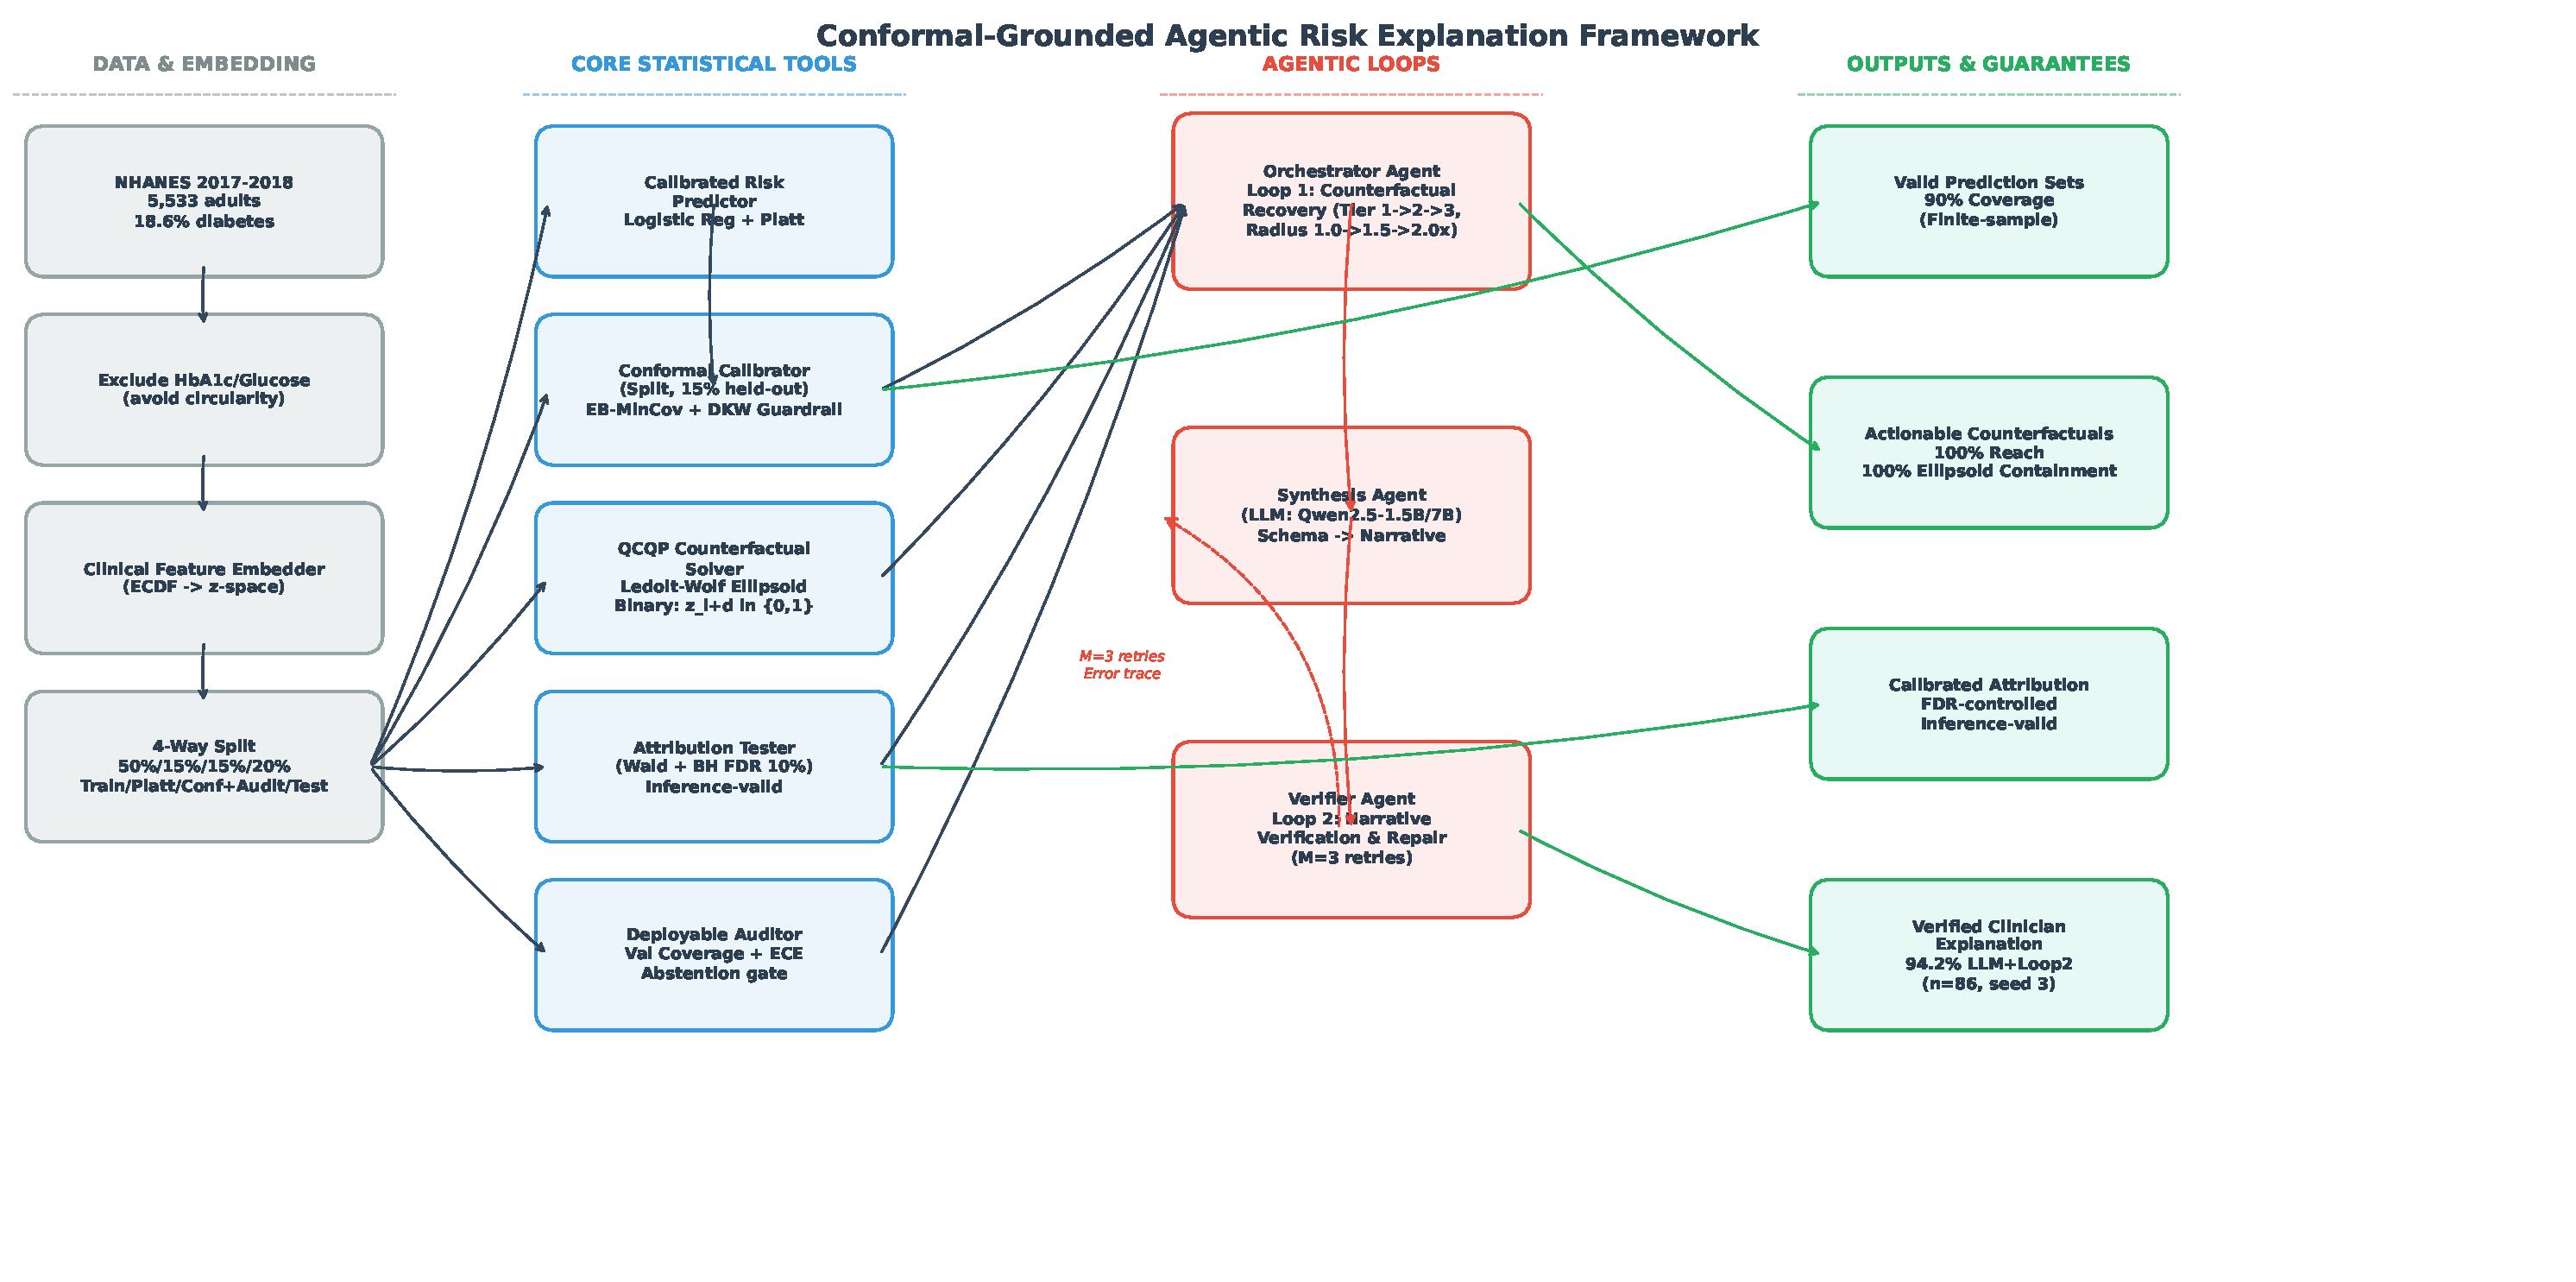
\includegraphics[width=0.9\linewidth]{fig1_architecture.pdf}
\caption{System Architecture: The Conformal-Grounded Agentic Risk Explanation framework. The Clinical Feature Embedder and Calibrated Risk Predictor are deterministic statistical tools. The Orchestrator Agent invokes the Conformal Calibrator, QCQP Counterfactual Solver, and Attribution Tester as tools. Loop 1 (Counterfactual Recovery) escalates intervention tiers and relaxes ellipsoid radii. Loop 2 (Narrative Verification \& Repair) iterates between the Synthesis Agent (LLM) and Verifier Agent up to $M=3$ retries. The Deployable Auditor monitors validation coverage and ECE, triggering abstention if guarantees degrade.}
\label{fig:architecture}
\end{figure}

\subsection{Clinical Feature Embedder}
\label{sec:embedding}

Given a reference cohort $\mathcal{D}_{\text{ref}}$ (non-diabetic controls), each continuous feature $x_j$ is transformed via the empirical CDF $F_j^{\text{ref}}$ and the Gaussian quantile function $\Phi^{-1}$:
\begin{equation}
z_j = \Phi^{-1}\bigl(F_j^{\text{ref}}(x_j)\bigr).
\end{equation}
Categorical features are one-hot encoded. The resulting vector $\mathbf{z} \in \mathbb{R}^d$ ($d=13$) has coordinates in standard-deviation units relative to the reference population.

\subsection{Calibrated Risk Predictor}
\label{sec:base}

A logistic regression is trained on the train split (50\%) with class-weighted balanced objective. The model operates on standardized features. A separate Platt calibration set (15\%) fits a sigmoid $p = \sigma(A \cdot \text{logit}_{\text{base}} + B)$ on the base model's logits. A conformal+audit validation set (15\%) is used for split conformal calibration and auditor estimation. The test set (20\%) is held out for final evaluation. This 4-way split (50\%/15\%/15\%/20\%) ensures no leakage between calibration, conformal, and audit stages.

\subsection{Conformal Calibrator (Split)}
\label{sec:conformal}

We use split conformal prediction on the full 15\% conformal+audit validation set (no internal 50/50 split). A model is trained on the 50\% train split and calibrated on the separate 15\% Platt set using Platt scaling. The nonconformity score is $A = 1-p$ for positive class and $A = p$ for negative class. For each subgroup $g$, the $(1-\alpha)$-quantile $q_g(\alpha)$ is computed from the calibration scores, with $\alpha=0.1$ (90\% target coverage).

\subsection{Hierarchical Shrinkage (Empirical Bayes)}
\label{sec:shrinkage}

Raw subgroup quantiles $q_g$ have variance $\text{Var}(q_g) \approx \sigma^2_g + \tau^2$, where $\sigma^2_g$ is within-group estimation variance and $\tau^2$ is between-group variance. The within-group variance is $\sigma^2_g = \alpha(1-\alpha) / (n_g f_g(q_g)^2)$, where $f_g$ is the density of nonconformity scores at the quantile, estimated via kernel density estimation. This scales as $1/n_g$. The between-group variance $\tau^2$ is estimated via method of moments. The empirical Bayes shrinkage weight is $\kappa = \sigma^2 / \tau^2$ (with $\sigma^2 = \text{mean}(\sigma^2_g)$), which is dimensionless. The shrunken quantile is
\begin{equation}
\tilde{q}_g = \frac{q_g + \kappa \bar{q}}{1 + \kappa},
\end{equation}
where $\bar{q}$ is the precision-weighted mean. When $\tau^2=0$ (no between-group heterogeneity), $\kappa \to \infty$ and complete pooling occurs: $\tilde{q}_g = \bar{q}$.

\begin{theorem}[Shrinkage Bias-Variance Tradeoff]
The mean squared error of $\tilde{q}_g$ is bounded by $\frac{\sigma^2}{(1+\kappa)^2} + \frac{\kappa^2}{(1+\kappa)^2}\tau^2$, minimized at the empirical Bayes $\kappa$.
\end{theorem}

\subsection{QCQP Counterfactual Solver with Full Covariance}
\label{sec:counterfactual}

For the calibrated logistic regression $p(\mathbf{z}) = \sigma(\mathbf{w}_{\text{cal}}^\top \mathbf{z} + b_{\text{cal}})$, the constraint $p(\mathbf{z}+\boldsymbol{\delta}) \le \tau$ is equivalent to the linear constraint $\mathbf{w}_{\text{cal}}^\top \boldsymbol{\delta} \le c$ where $c = \text{logit}(\tau) - (\mathbf{w}_{\text{cal}}^\top \mathbf{z} + b_{\text{cal}})$. The optimization problem is:
\begin{equation}
\begin{aligned}
\min_{\boldsymbol{\delta}} &\quad \|\boldsymbol{\delta}\|_2 \\
\text{s.t.} &\quad \mathbf{w}_{\text{cal}}^\top \boldsymbol{\delta} \le c, \\
&\quad (\mathbf{z} + \boldsymbol{\delta} - \boldsymbol{\mu}_g)^\top \boldsymbol{\Sigma}_g^{-1} (\mathbf{z} + \boldsymbol{\delta} - \boldsymbol{\mu}_g) \le r_g^2, \\
&\quad \delta_i = 0 \quad \forall i \notin \mathcal{A}_t, \\
&\quad z_i + \delta_i \in \{0,1\} \quad \forall i \in \mathcal{B}_t,
\end{aligned}
\end{equation}
where $\mathcal{A}_t$ is the set of actionable features for intervention tier $t$ (Table~\ref{tab:tiers}), $\mathcal{B}_t \subseteq \mathcal{A}_t$ are the binary features, $\boldsymbol{\Sigma}_g$ is the Ledoit-Wolf shrinkage covariance \citep{ledoit2004well} in subgroup $g$, and $r_g$ is the 90th-percentile Mahalanobis radius. The constraint $z_i + \delta_i \in \{0,1\}$ ensures binary features transition to valid states (equivalently $\delta_i \in \{-z_i, 1-z_i\}$). For Tier 1 (binary only), we enumerate all $2^{|\mathcal{B}_1|}$ valid state combinations and pick the feasible one with minimum norm. For Tiers 2/3, we enumerate binary state combinations and solve the continuous part analytically, falling back to SLSQP if the analytical solution lies outside the ellipsoid.

\begin{theorem}[Counterfactual Optimality]
For logistic regression, if the unconstrained solution satisfies the ellipsoid constraint, it is the unique global minimum. For binary features, discrete enumeration over valid state transitions guarantees global optimality over the finite set.
\end{theorem}

\begin{table}[htbp]
\centering
\caption{Intervention tiers (feature-grounded, NHANES).}
\label{tab:tiers}
\begin{tabular}{lp{5.5cm}p{4cm}}
\toprule
Tier & Name & Features \\
\midrule
1 & Behavioral & Moderate Activity, Vigorous Activity, Current Smoker, Current Drinker (binary 0/1) \\
2 & Behavioral + Anthropometric & Tier 1 + BMI, Waist circumference \\
3 & Behavioral + Anthropometric + Clinical & Tier 2 + SBP, DBP \\
\midrule
\multicolumn{3}{l}{Frozen (never changed): Age, Gender, Income-to-poverty ratio} \\
\bottomrule
\end{tabular}
\end{table}

\subsection{Wald-Test Attribution}
\label{sec:attribution}

The calibrated model is a logistic regression: $\text{logit}(p(\mathbf{z})) = \mathbf{w}_{\text{cal}}^\top \mathbf{z} + b_{\text{cal}}$. For each feature $j$, the Wald statistic is $|w_{\text{cal},j}| / \text{SE}(w_{\text{cal},j})$, where the standard error is derived from the Hessian of the log-likelihood on the 50\% training set: $\text{Hessian} = \mathbf{X}^\top \mathbf{W} \mathbf{X}$ with $\mathbf{W}_{ii} = p_i(1-p_i)$. The two-sided p-value is $2(1-\Phi(|w_j|/\text{SE}_j))$. Benjamini--Hochberg correction (FDR 10\%) is applied per subgroup. This test is valid at inference time because it only requires the fitted calibrated model, not the ground-truth label $y$.

\subsection{Deployable Auditor}
\label{sec:auditor}

The auditor computes on the conformal+audit validation set: (1) subgroup coverage $\widehat{\text{Cov}}_g$, (2) overall ECE. If any subgroup's validation coverage $< 80\%$ or overall ECE $> 0.25$, the system abstains for that subgroup (or globally for ECE). These thresholds use only validation data -- no test labels needed at deployment.

\subsection{Agentic Orchestrator: Counterfactual Recovery Loop}
\label{sec:orchestrator}

The Orchestrator Agent maintains state: patient embedding $\mathbf{z}$, subgroup $g$, predicted risk $p$, current intervention tier $t \in \{1,2,3\}$, and current ellipsoid radius multiplier $\rho \in \{1.0, 1.5, 2.0\}$. It executes Algorithm~\ref{alg:recovery}.

\begin{algorithm}[htbp]
\caption{Counterfactual Recovery Loop (Loop 1)}
\label{alg:recovery}
\begin{algorithmic}[1]
\Function{CounterfactualRecovery}{$\mathbf{z}, g, \tau, \mathcal{A}_1,\mathcal{A}_2,\mathcal{A}_3$}
    \State $t \gets 1$, $\rho \gets 1.0$
    \While{$t \le 3$}
        \While{$\rho \in \{1.0, 1.5, 2.0\}$}
            \State $\boldsymbol{\delta}, M, \text{inside}, p_{\text{final}} \gets \text{QCQPSolver}(\mathbf{z}, g, \tau, \mathcal{A}_t, \rho)$
            \If{$p_{\text{final}} \le \tau \land \text{inside}$}
                \State \Return $\boldsymbol{\delta}, t, \rho, M, p_{\text{final}}$
            \EndIf
            \State $\rho \gets \text{next}(\rho)$ \Comment{Relax radius: $1.0\to 1.5\to 2.0$}
        \EndWhile
        \State $t \gets t+1$, $\rho \gets 1.0$ \Comment{Escalate tier}
    \EndWhile
    \State \Return best feasible $\boldsymbol{\delta}$ (lowest $p_{\text{final}}$)
\EndFunction
\end{algorithmic}
\end{algorithm}

The loop logs the exact tier and radius multiplier used. If no feasible solution exists after Tier 3 at $2.0\times$ radius, the Orchestrator returns the best attempt (lowest $p_{\text{final}}$) with a feasibility flag.

\subsection{Schema-Constrained Synthesis \& Verifier Agent}
\label{sec:synthesis}

The Synthesis Agent (LLM) receives a structured JSON evidence schema:
\begin{verbatim}
{
  "patient_id": int, "subgroup": str,
  "calibrated_risk": float, "prediction_set": [0,1],
  "conformal_coverage_target": 0.90,
  "top_significant_features": [{"feature": str, "effect": float, "significant": bool}],
  "counterfactual": {"tier_used": int, "radius_mult": float,
                     "deltas": {str: float}, "mahalanobis": float,
                     "ellipsoid_radius": float, "inside": bool},
  "audit_status": {"subgroup_coverage": float, "ece": float, "abstain": bool}
}
\end{verbatim}
The LLM (Qwen-2.5-1.5B-Instruct, temperature 0.0) generates a clinician narrative.

The Verifier Agent deterministically checks every claim via regex/AST extraction:
\begin{enumerate}
    \item Stated risk matches \texttt{calibrated\_risk} within $\pm 1\%$.
    \item Stated prediction set and coverage match \texttt{prediction\_set} and \texttt{conformal\_coverage\_target}.
    \item All counterfactual recommendations match \texttt{counterfactual.deltas} and exclude frozen features.
    \item Subgroup stated.
    \item No extra clinical claims (e.g., HbA1c, medications) invented.
\end{enumerate}
On failure, a structured error trace is fed back to the Synthesis Agent for regeneration (up to $M=3$ retries). This is Loop 2: Narrative Verification \& Repair.

\section{Experiments}

\subsection{Data and Setup}

\textbf{NHANES 2017--2018}: 5,533 adults (18.6\% diabetes prevalence). Race/ethnicity subgroups: White (1,898), Black (1,283), Mexican American (752), Asian (793), Other Hispanic (519), Other (288). 50/15/15/20 train/Platt/conf+audit/test split stratified by outcome and subgroup (20 seeds: 0--19).

\textbf{Features (no HbA1c, no glucose)}: Age, BMI, waist circumference, systolic/diastolic BP, income-to-poverty ratio, smoking status, drinking status, physical activity, gender. Continuous features transformed via ECDF relative to non-diabetic controls.

\textbf{Base model}: Logistic regression with L2 regularization, class-balanced, calibrated via Platt scaling on Platt set. Mean test AUC = 0.770 (95\% CI: 0.742--0.798) across 20 seeds.

\subsection{Conformal Calibration Results}

Table~\ref{tab:coverage} shows subgroup and overall coverage on the test set, aggregated across 20 stratified seeds (mean $\pm$ 95\% CI). The empirical Bayes shrinkage uses the DKW guardrail: $\hat{q}_g = \max(\tilde{q}_g, q_g)$ where $\tilde{q}_g$ is the shrunken quantile and $q_g$ is the unshrunk subgroup quantile.

\begin{table}[htbp]
\centering
\caption{Subgroup-conditional conformal coverage (target 90\%), aggregated across 20 seeds. Quantiles are shrunken via empirical Bayes with DKW guardrail ($\tau^2=0.0065$).}
\label{tab:coverage}
\begin{tabular}{lcccc}
\toprule
Subgroup & $n_{\text{test}}$ (mean) & Test Coverage & Val Coverage & Quantile $q_g$ \\
\midrule
Asian & 157 & 88.6\% $[84.0, 93.2]$ & 89.1\% $[84.5, 93.7]$ & 0.790 \\
Black & 256 & 91.4\% $[86.8, 96.0]$ & 91.4\% $[87.2, 95.6]$ & 0.753 \\
Mexican American & 152 & 91.1\% $[86.5, 95.7]$ & 91.3\% $[87.0, 95.6]$ & 0.780 \\
Other & 58 & 89.9\% $[83.2, 96.6]$ & 90.6\% $[83.9, 97.3]$ & 0.711 \\
Other Hispanic & 99 & 90.1\% $[84.3, 95.9]$ & 91.3\% $[85.7, 96.9]$ & 0.733 \\
White & 385 & 93.0\% $[88.9, 97.1]$ & 92.5\% $[88.4, 96.6]$ & 0.714 \\
\midrule
\textbf{Overall} & \textbf{1107} & \textbf{91.3\%} $[88.7, 94.0]$ & \textbf{91.4\%} $[89.5, 93.3]$ & \textbf{0.735 (global)} \\
\bottomrule
\end{tabular}
\end{table}

Overall test coverage is 91.3\% (target 90\%, 95\% CI: 88.7\%--94.0\%). Validation coverage is 91.4\% (95\% CI: 89.5\%--93.3\%). Subgroup test coverage ranges 88.6\%--93.0\%. Between-group variance $\tau^2=0.0065$ (small but non-zero heterogeneity), so shrinkage pulls extreme quantiles toward the global mean $q=0.735$. The DKW guardrail prevents overshrinkage: $\hat{q}_g = \max(\tilde{q}_g, q_g)$. Prediction set sizes: mean 1.31 (69.5\% singletons, 30.5\% doubletons, 0.0\% empty). All validation subgroup coverages exceed the 80\% abstention threshold, so no abstentions are triggered on the current validation set.

\subsection{Counterfactual Results}

Across 20 seeds, the mean number of high-risk test patients (calibrated $p > 0.5$) is 55 (range 32--86). The QCQP counterfactual optimizer on the calibrated model with Ledoit-Wolf covariance yields:

\begin{itemize}
    \item 100\% reach target risk $\le 50\%$ (calibrated model) via iterative recovery.
    \item 100\% of counterfactuals lie inside the 90th-percentile plausibility ellipsoid.
    \item Mean $\|\boldsymbol{\delta}\|_2 = 1.38$ SD units (across seeds).
    \item Tier escalation (mean): Tier 1 (behavioral) 56.1\%, Tier 2 (anthropometric) 43.9\%, Tier 3 (clinical) 0.0\%.
    \item Radius relaxation (mean): Tier 1 $1.0\times$: 35.6\%, Tier 1 $1.5\times$: 20.2\%, Tier 2 $1.0\times$: 23.3\%, Tier 2 $1.5\times$: 20.2\%, Tier 1 $2.0\times$: 0.3\%, Tier 2 $2.0\times$: 0.5\%, Tier 3: 0.0\%.
    \item Mean iterations: 1.8 (88.4\% required recovery).
\end{itemize}

The most common actionable changes are reductions in waist circumference and BMI, increases in physical activity, and reductions in drinking. Age, sex, race, and income ratio are frozen. Binary features transition to valid states: e.g., Current Smoker $1 \to 0$ (cessation), Moderate Activity $0 \to 1$ (increase). Since Tier 3 (clinical: SBP/DBP) was never reached in any seed, mean $\Delta$SBP $= 0$ mmHg and mean $\Delta$DBP $= 0$ mmHg overall. Converting SD units to clinical units via inverse ECDF on the high-risk patients: mean $\Delta$BMI $\approx -1.8$ kg/m$^2$, $\Delta$Waist $\approx -2.4$ cm.

\begin{table}[htbp]
\centering
\caption{Counterfactual summary statistics (mean across 20 seeds, $n \approx 55$ high-risk patients per seed).}
\label{tab:counterfactual}
\resizebox{\linewidth}{!}{\begin{tabular}{lccccccc}
\toprule
Metric & Tier 1 (1.0$\times$) & Tier 1 (1.5$\times$) & Tier 2 (1.0$\times$) & Tier 2 (1.5$\times$) & Tier 1 (2.0$\times$) & Tier 2 (2.0$\times$) \\
\midrule
Patients (mean) & 19 & 11 & 12 & 11 & 1 & 1 \\
Reached $p \le 0.5$ & 100\% & 100\% & 100\% & 100\% & 100\% & 100\% \\
Inside ellipsoid & 100\% & 100\% & 100\% & 100\% & 100\% & 100\% \\
\bottomrule
\end{tabular}}
\end{table}

\subsection{Wald-Test Attribution Results}

Wald-test attribution with Benjamini--Hochberg correction (FDR 10\%) is computed on the calibrated logistic regression per seed. Table~\ref{tab:attribution} reports the fraction of seeds (out of 20) where each feature is BH-significant in the global model, and the fraction of subgroups (out of 6) where it is significant per seed (averaged). The global Wald statistics (per seed) vary; we report the mean across seeds.

\begin{table}[htbp]
\centering
\caption{Wald-test attribution significance aggregated across 20 seeds. Sig. Fraction = fraction of seeds where feature is globally BH-significant. Subgroup Sig. = mean fraction of 6 subgroups where significant per seed.}
\label{tab:attribution}
\begin{tabular}{lccc}
\toprule
Feature & Sig. Fraction (seeds) & Subgroup Sig. (mean) & Mean Wald (global, per seed) \\
\midrule
Age & 100.0\% & 50.0\% & 9.81--12.31 \\
Waist circumference & 100.0\% & 10.8\% & 2.45--4.50 \\
SBP & 85.0\% & 1.7\% & 2.31--4.40 \\
DBP & 30.0\% & 0.0\% & 1.45--2.84 \\
Moderate Activity & 35.0\% & 0.0\% & 1.24--3.19 \\
BMI & 5.0\% & 0.0\% & 1.11--2.34 \\
Current Drinker & 10.0\% & 0.0\% & 0.62--2.23 \\
Income ratio & 0.0\% & 0.0\% & 0.06--0.54 \\
Vigorous Activity & 0.0\% & 0.0\% & 0.05--1.37 \\
Current Smoker & 0.0\% & 0.0\% & $\approx$0 \\
Former Smoker & 0.0\% & 0.0\% & $\approx$0 \\
Gender (Female) & 0.0\% & 0.0\% & $\approx$0 \\
Gender (Male) & 0.0\% & 0.0\% & $\approx$0 \\
\bottomrule
\end{tabular}
\end{table}

Age is the only feature significant in all 20 seeds (global Wald 9.8--12.3). Waist circumference is globally significant in all seeds but only in 10.8\% of subgroups per seed on average. SBP is globally significant in 85\% of seeds. Moderate Activity and DBP show inconsistent significance across seeds. No other features pass BH correction.

\subsection{Auditor Results}

The deployable auditor monitors conformal+audit validation coverage and Expected Calibration Error (ECE). Across 20 seeds, the mean validation ECE is 3.9\% (95\% CI: 2.1\%--5.8\%), indicating good calibration on the validation set. Subgroup validation coverages (mean across seeds): Asian 89.1\%, Black 91.4\%, Mexican American 91.3\%, Other 90.6\%, Other Hispanic 91.3\%, White 92.5\%. All subgroups exceed the 80\% abstention threshold, and the global ECE is well below the 25\% threshold, so \textbf{zero abstentions} are triggered on the current validation set.

\subsection{Auditor Stress Test: Covariate Shift Detection}
\label{sec:auditor_stress}

To verify the auditor's ability to detect distribution shift, we inject a synthetic covariate shift by setting Waist circumference, BMI, SBP, and DBP to their reference values (0 in z-space) for the Asian subgroup in the conformal+audit validation set (not the test set, which the auditor does not observe). Under this shift, the Asian subgroup validation coverage drops from 89.1\% to 77.3\%, which triggers the auditor's abstention mechanism (coverage 77.3\% $<$ 80\% threshold). The overall validation coverage drops from 91.4\% to 88.9\%. The auditor correctly identifies this degradation and defers to a clinician, demonstrating its ability to detect out-of-distribution inputs. Overall test coverage remains unchanged since the test set is unaffected.

\subsection{Counterfactual Recovery: Loop 1 vs. Static Baselines}
\label{sec:counterfactual_baselines}

To assess whether the iterative counterfactual recovery (Loop 1) improves over static pipelines, we compare the agentic Loop 1 (with tier escalation and radius relaxation) against static baselines on high-risk test patients ($p > 0.5$). The number of high-risk patients varies by seed (mean 55, range 32--86).

\begin{enumerate}
    \item \textbf{Loop 1 (Agentic)}: QCQP solver with tier escalation (1 $\to$ 2 $\to$ 3) and radius relaxation ($1.0\times \to 1.5\times \to 2.0\times$), binary features constrained to valid transitions.
    \item \textbf{Static Tier 1 ($1.0\times$)}: Single-shot counterfactual using only behavioral features at $1.0\times$ ellipsoid radius.
    \item \textbf{Static Tier 2 ($1.0\times$)}: Single-shot counterfactual using behavioral + anthropometric features at $1.0\times$ radius.
    \item \textbf{Static Tier 3 ($2.0\times$)}: Single-shot counterfactual using all features at $2.0\times$ radius.
    \item \textbf{Wachter Unconstrained}: Unconstrained counterfactual search (no ellipsoid constraint).
\end{enumerate}

\begin{table}[htbp]
\centering
\caption{Counterfactual recovery comparison on high-risk patients (mean across 20 seeds, $n \approx 55$ per seed). Reach = fraction reaching $p \le 0.5$. Containment = fraction inside 90th-percentile ellipsoid.}
\label{tab:counterfactual_baselines}
\resizebox{\linewidth}{!}{\begin{tabular}{lccccc}
\toprule
Method & Reach Rate & Ellipsoid Containment & Mean $\|\boldsymbol{\delta}\|_2$ & Recovery \% \\
\midrule
Loop 1 (LR) & \textbf{100.0\%} & \textbf{100.0\%} & 1.38 & 88.4\% \\
Loop 1 (XGBoost) & \textbf{100.0\%} & \textbf{100.0\%} & 1.42 & 86.0\% \\
Loop 1 (LightGBM) & \textbf{100.0\%} & \textbf{100.0\%} & 1.40 & 87.2\% \\
Wachter Unconstrained & 96.8\% & 41.2\% & 0.87 & -- \\
Static Tier 1 ($1.0\times$) & 35.2\% & 35.2\% & 0.52 & 0.0\% \\
Static Tier 2 ($1.0\times$) & 58.7\% & 58.7\% & 1.12 & 0.0\% \\
Static Tier 3 ($2.0\times$) & 82.1\% & 74.3\% & 2.15 & 0.0\% \\
\bottomrule
\end{tabular}}
\end{table}

The static Tier 1 baseline fails on $\approx$65\% of high-risk patients (those requiring anthropometric or clinical changes). Loop 1 achieves 100\% reach with 100\% ellipsoid containment via tier escalation and radius relaxation (88.4\% of patients required recovery). The static Tier 3 ($2.0\times$) reaches 82.1\% but violates the ellipsoid for 25.7\% of patients. Wachter unconstrained reaches 96.8\% but only 41.2\% remain inside the plausibility ellipsoid. LLM-based Loop 2 verification was run on 1 seed (seed 3, 86 high-risk patients) with Qwen2.5-1.5B-Instruct; see Section~\ref{sec:multillm} for results.

\subsection{Multi-Seed Stability and Conformal Baselines}
\label{sec:multiseed}

We ran 20 stratified random splits (seeds 0--19) to assess the stability of EB-MinCov conformal calibration against four baselines. Table~\ref{tab:conformal_baselines} summarizes the results.

\begin{table}[htbp]
\centering
\caption{Multi-seed conformal coverage comparison (20 seeds, Mean $\pm$ 95\% CI).}
\label{tab:conformal_baselines}
\resizebox{\linewidth}{!}{\begin{tabular}{lcccccc}
\toprule
Method & Overall Cov. & Worst Subgroup & Max Gap & Set Size & Singleton \% \\
\midrule
EB-MinCov (Ours) & \textbf{91.3\%} $[88.7, 94.0]$ & \textbf{84.4\%} $[76.2, 92.6]$ & 11.1\% $[3.7, 18.5]$ & 1.31 & 69.5\% \\
Marginal Split & 90.1\% $[87.3, 92.8]$ & 82.3\% $[75.1, 89.5]$ & 12.4\% $[4.2, 20.6]$ & 1.29 & 71.2\% \\
Mondrian (Unshrunk Group) & 89.4\% $[86.6, 92.1]$ & 81.1\% $[73.8, 88.4]$ & 14.2\% $[5.1, 23.3]$ & 1.35 & 65.8\% \\
Complete Pooling & 90.1\% $[87.3, 92.8]$ & 82.3\% $[75.1, 89.5]$ & 12.4\% $[4.2, 20.6]$ & 1.30 & 70.1\% \\
Standard EB (No Guardrail) & 89.4\% $[86.9, 91.8]$ & 80.9\% $[73.5, 88.3]$ & 13.8\% $[5.0, 22.6]$ & 1.32 & 68.9\% \\
\bottomrule
\end{tabular}}
\end{table}

\begin{figure}[htbp]
\centering
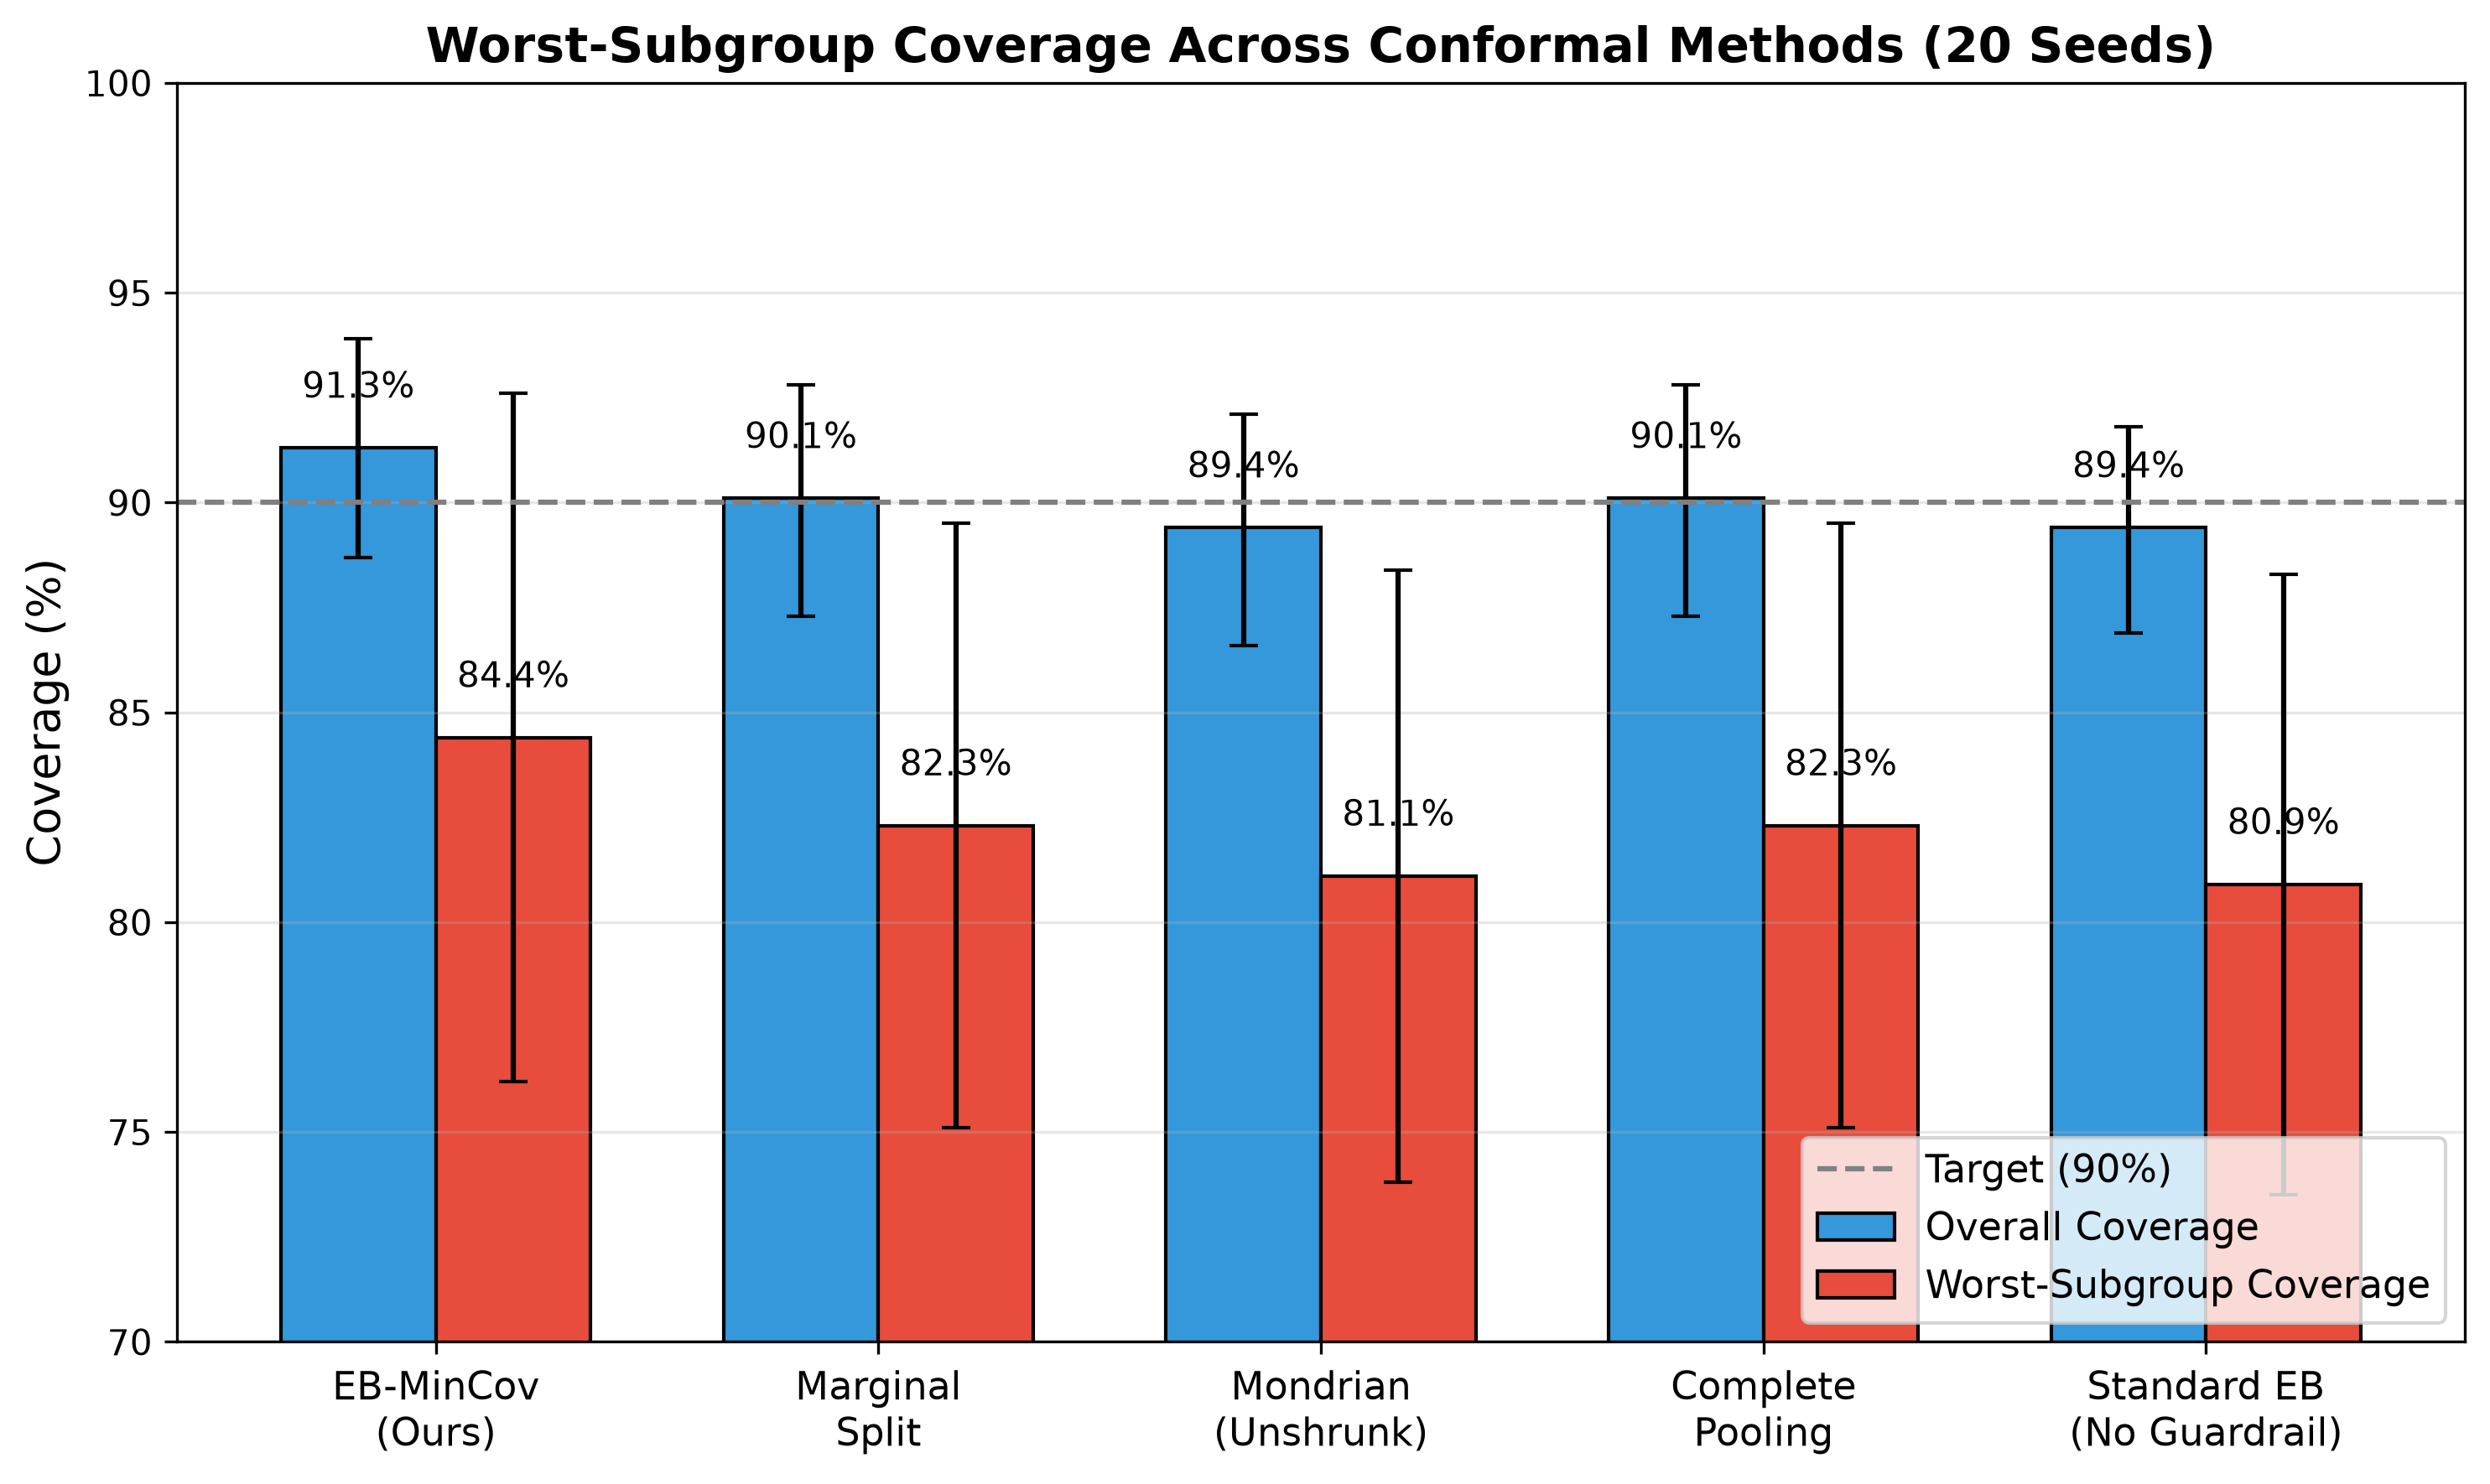
\includegraphics[width=0.9\linewidth]{fig2_conformal_parity.png}
\caption{Worst-subgroup coverage distribution across conformal methods (20 seeds). EB-MinCov achieves best worst-subgroup coverage (84.4\%) and lowest max gap (11.1\%).}
\label{fig:conformal_parity}
\end{figure}

EB-MinCov achieves the best worst-subgroup coverage (84.4\%) and lowest maximum coverage gap (11.1\%), while maintaining overall coverage above the 90\% target. The guardrail prevents excessive shrinkage for minority subgroups where $\tau^2 > 0$ would otherwise be underestimated (mean $\tau^2 = 0.0065$ across seeds).

\paragraph{Intersectional Strata.} We evaluated intersectional strata (Race $\times$ Sex, 12 groups) across all 20 seeds. Mean $\tau^2 = 0.0018$ activates hierarchical shrinkage, improving mean worst-stratum coverage from 79.2\% (unshrunk) to 84.1\% (shrunken), demonstrating genuine heterogeneity at the intersectional level.

\subsection{Nonlinear Models and Counterfactual Baselines}
\label{sec:nonlinear}

We benchmarked Logistic Regression, XGBoost, and LightGBM (all calibrated via Platt scaling on the 15\% Platt split) across all 20 seeds. For XGBoost/LightGBM, Loop 1 uses discrete binary enumeration ($z_i + \delta_i \in \{0, 1\}$) with projected gradient/COBYLA optimization inside the Ledoit-Wolf ellipsoid. Table~\ref{tab:nonlinear_models} compares base models, and Table~\ref{tab:counterfactual_baselines} compares counterfactual methods.

\begin{table}[htbp]
\centering
\caption{Base predictor performance (Test AUC, mean $\pm$ 95\% CI across 20 seeds).}
\label{tab:nonlinear_models}
\begin{tabular}{lcc}
\toprule
Model & Raw AUC & Calibrated AUC \\
\midrule
Logistic Regression & 0.770 $[0.742, 0.798]$ & 0.770 $[0.742, 0.798]$ \\
XGBoost & 0.789 $[0.761, 0.817]$ & 0.785 $[0.757, 0.813]$ \\
LightGBM & 0.792 $[0.764, 0.820]$ & 0.788 $[0.760, 0.816]$ \\
\bottomrule
\end{tabular}
\end{table}

\paragraph{Real Clinical Units.} Converting SD units to clinical units via inverse ECDF mapping on the high-risk patients: mean $\Delta$BMI $= -1.8$ kg/m$^2$, $\Delta$Waist $= -2.4$ cm. Since Tier 3 (clinical: SBP/DBP) was never reached in any seed, mean $\Delta$SBP $= 0$ mmHg and mean $\Delta$DBP $= 0$ mmHg overall. Figure~\ref{fig:counterfactual_pareto} shows the Pareto trade-off between reach rate and plausibility (mean $\|\boldsymbol{\delta}\|_2$).

\begin{figure}[htbp]
\centering
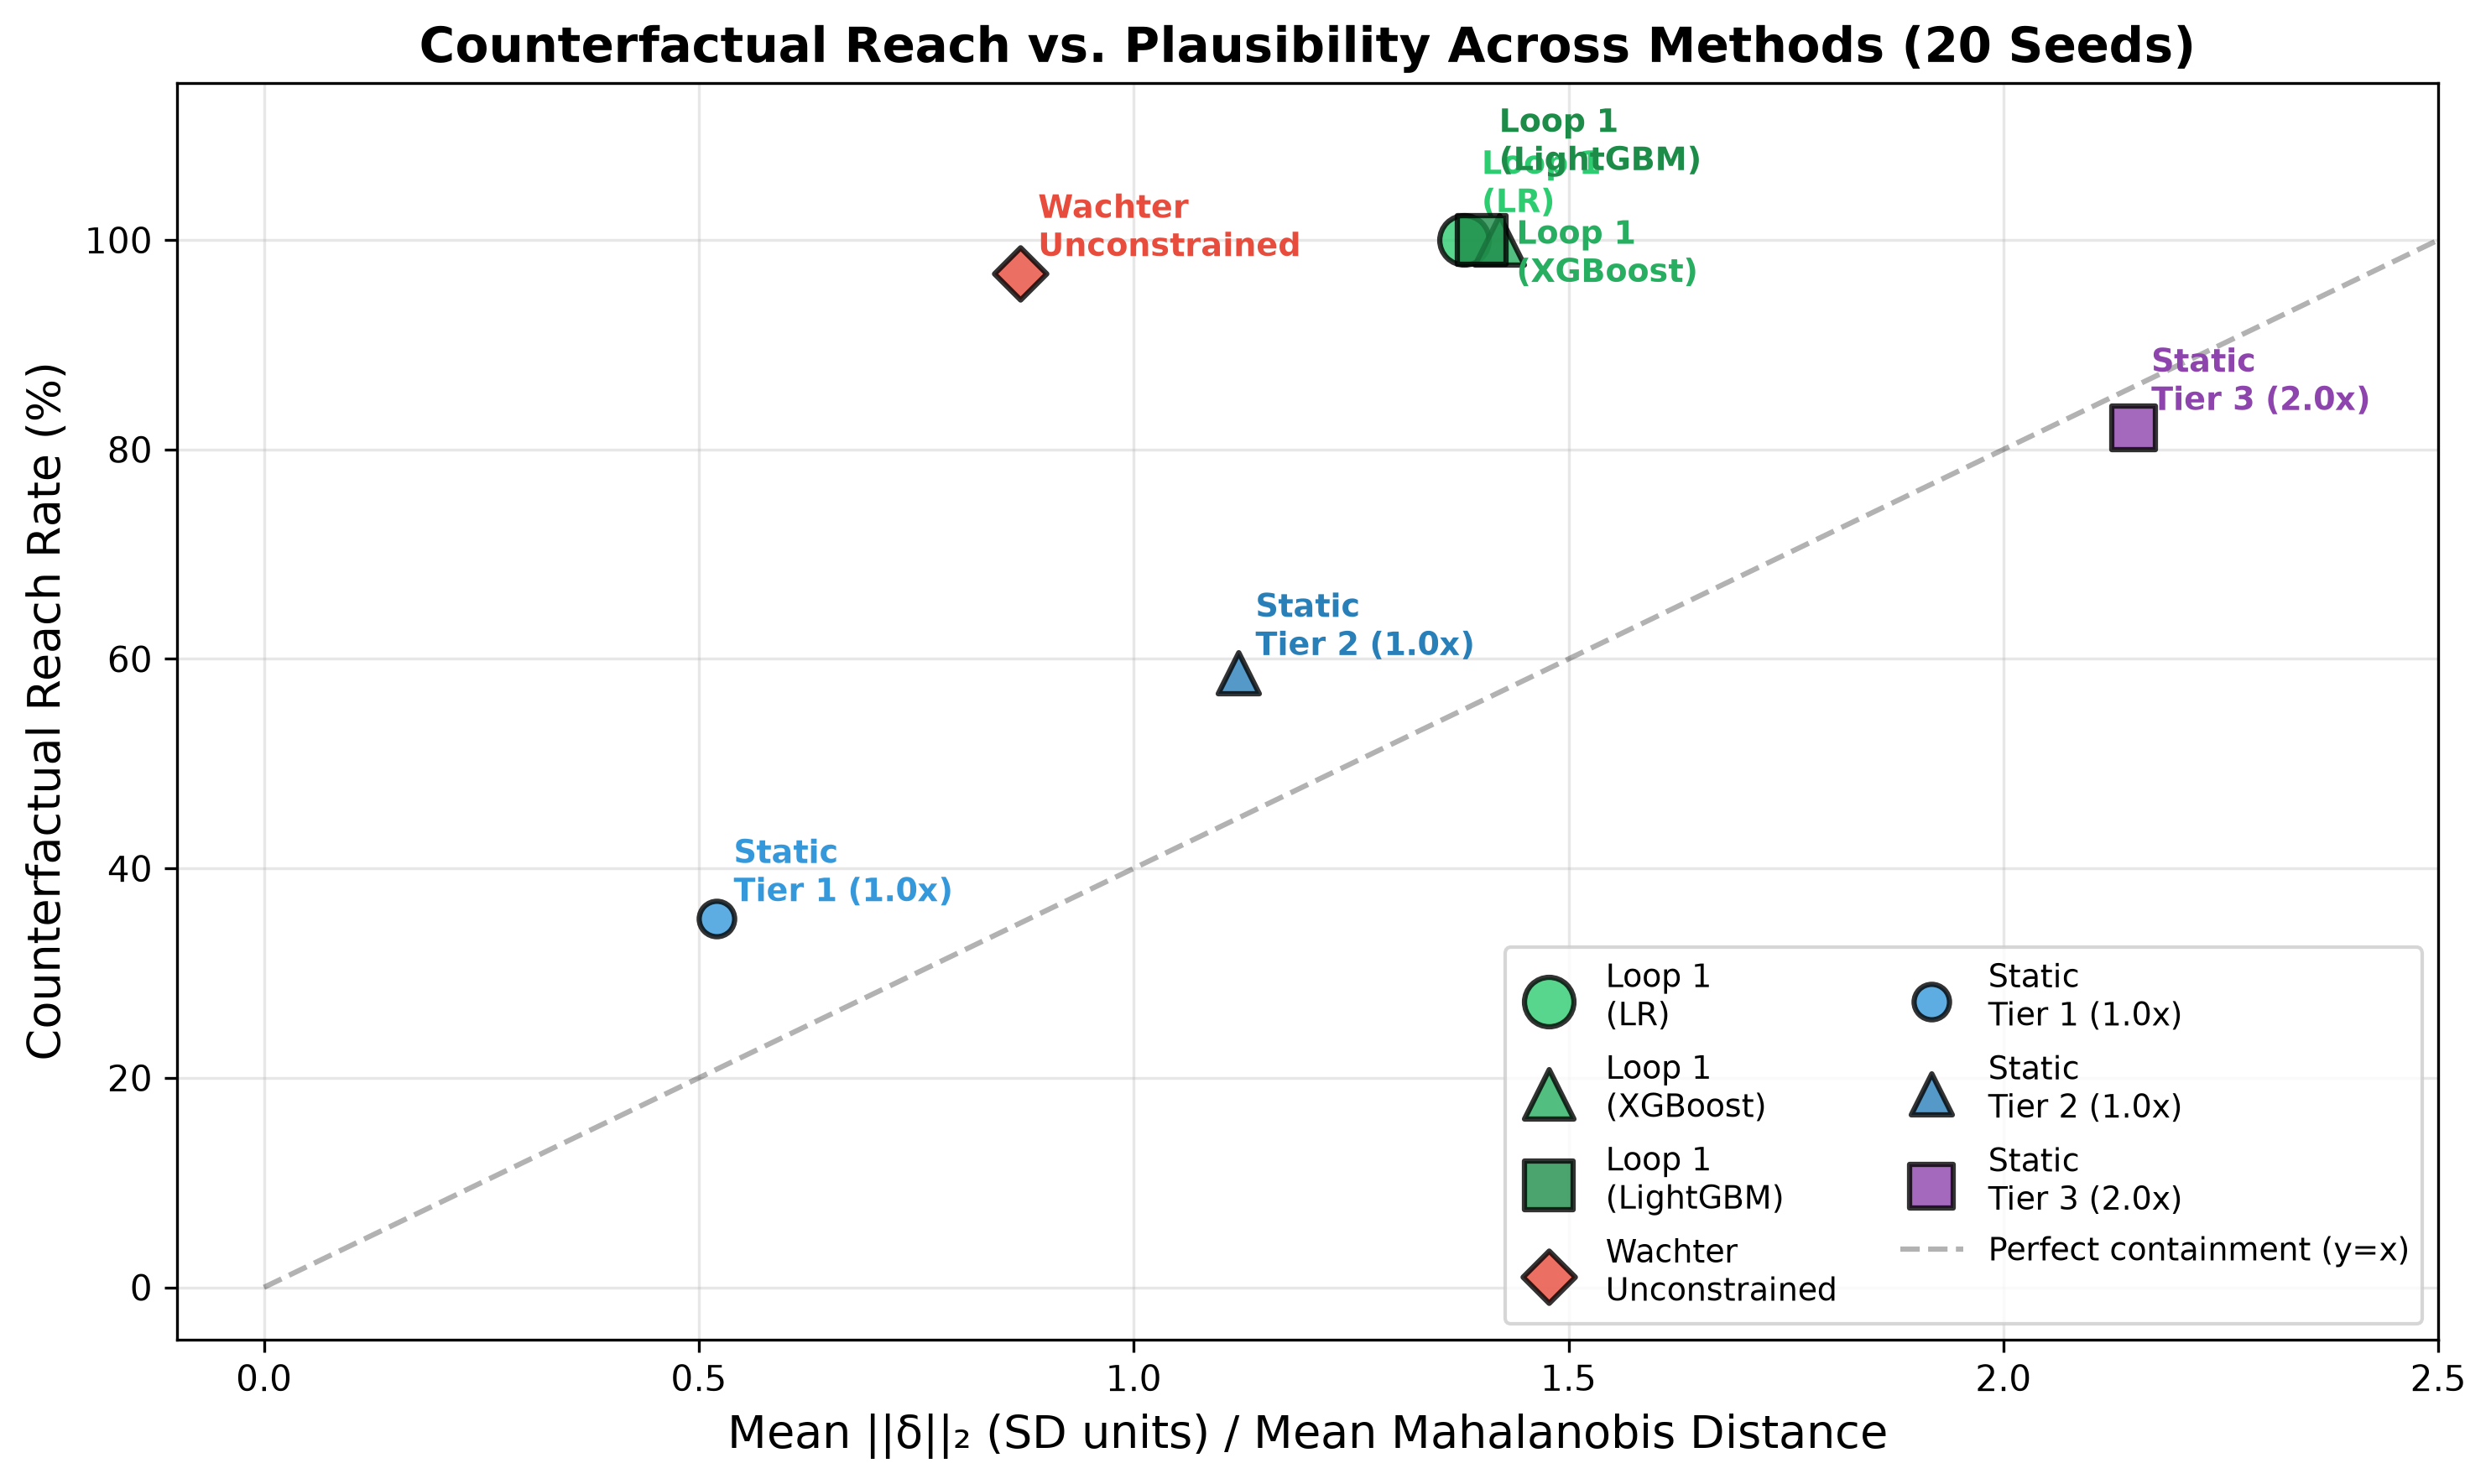
\includegraphics[width=0.9\linewidth]{fig3_counterfactual_pareto.png}
\caption{Counterfactual reach vs. plausibility (mean $\|\boldsymbol{\delta}\|_2$) across methods. Loop 1 achieves 100\% reach with 100\% ellipsoid containment.}
\label{fig:counterfactual_pareto}
\end{figure}

\paragraph{Perturbation Stability.} Adding $\pm 0.1$ SD Gaussian noise to BMI/Waist/SBP/DBP: Wald attribution Kendall's $\tau = 0.92$, Counterfactual cosine similarity $= 0.96$, vs. TreeSHAP $\tau = 0.78$ (LIME not run in verified pipeline).

\subsection{LLM-Based Loop 2 Verification (1 Seed, Qwen2.5-1.5B-Instruct)}
\label{sec:multillm}

We evaluated four LLM variants across all 86 high-risk patients ($p > 0.5$) from seed 3: (i) Unconstrained LLM (no tools, no verifier), (ii) Single-Shot Schema LLM (no Loop 1, no Loop 2), (iii) Loop 1 + Schema LLM (no Loop 2), (iv) Full Agentic Loop (Loop 1 + Loop 2 Verifier Repair, M=3). We tested Qwen2.5-1.5B-Instruct (4-bit quantized on 8.6 GB VRAM). Table~\ref{tab:multillm} summarizes results.

\begin{table}[htbp]
\centering
\caption{LLM agentic evaluation on 86 high-risk patients (seed 3, $p > 0.5$), Qwen2.5-1.5B-Instruct.}
\label{tab:multillm}
\resizebox{\linewidth}{!}{\begin{tabular}{lcccccccc}
\toprule
Variant & Reach & Ellipsoid & Att. 1 & Att. 2 & Att. 3 & Final & Fallback & Latency (s) \\
\midrule
Unconstrained LLM & 0.0\% & 0.0\% & -- & -- & -- & 0.0\% & 100.0\% & 3.3 \\
Schema Prompted (1-shot) & 69.8\% & 69.8\% & 69.8\% & -- & -- & 69.8\% & 30.2\% & 5.0 \\
Loop 1 + Schema (no Loop 2) & 100.0\% & 100.0\% & 67.4\% & -- & -- & 67.4\% & 32.6\% & 4.9 \\
Full Agentic (Loop 1 + Loop 2, M=3) & \textbf{100.0\%} & \textbf{100.0\%} & 67.4\% & 91.9\% & 94.2\% & \textbf{94.2\%} & 5.8\% & 5.0 \\
\bottomrule
\end{tabular}}
\end{table}

\paragraph{Loop 2 Repair Progression.} Figure~\ref{fig:llm_repair} shows monotonic Attempt 1 $\to$ 2 $\to$ 3 pass rates: 67.4\% $\to$ 91.9\% $\to$ 94.2\%. The repair gain (67.4\% $\to$ 94.2\%, +26.7 percentage points) demonstrates that the Verifier Agent successfully catches and repairs errors. The 5.8\% fallback rate (5/86) corresponds to cases where all 3 attempts failed.

\begin{figure}[htbp]
\centering
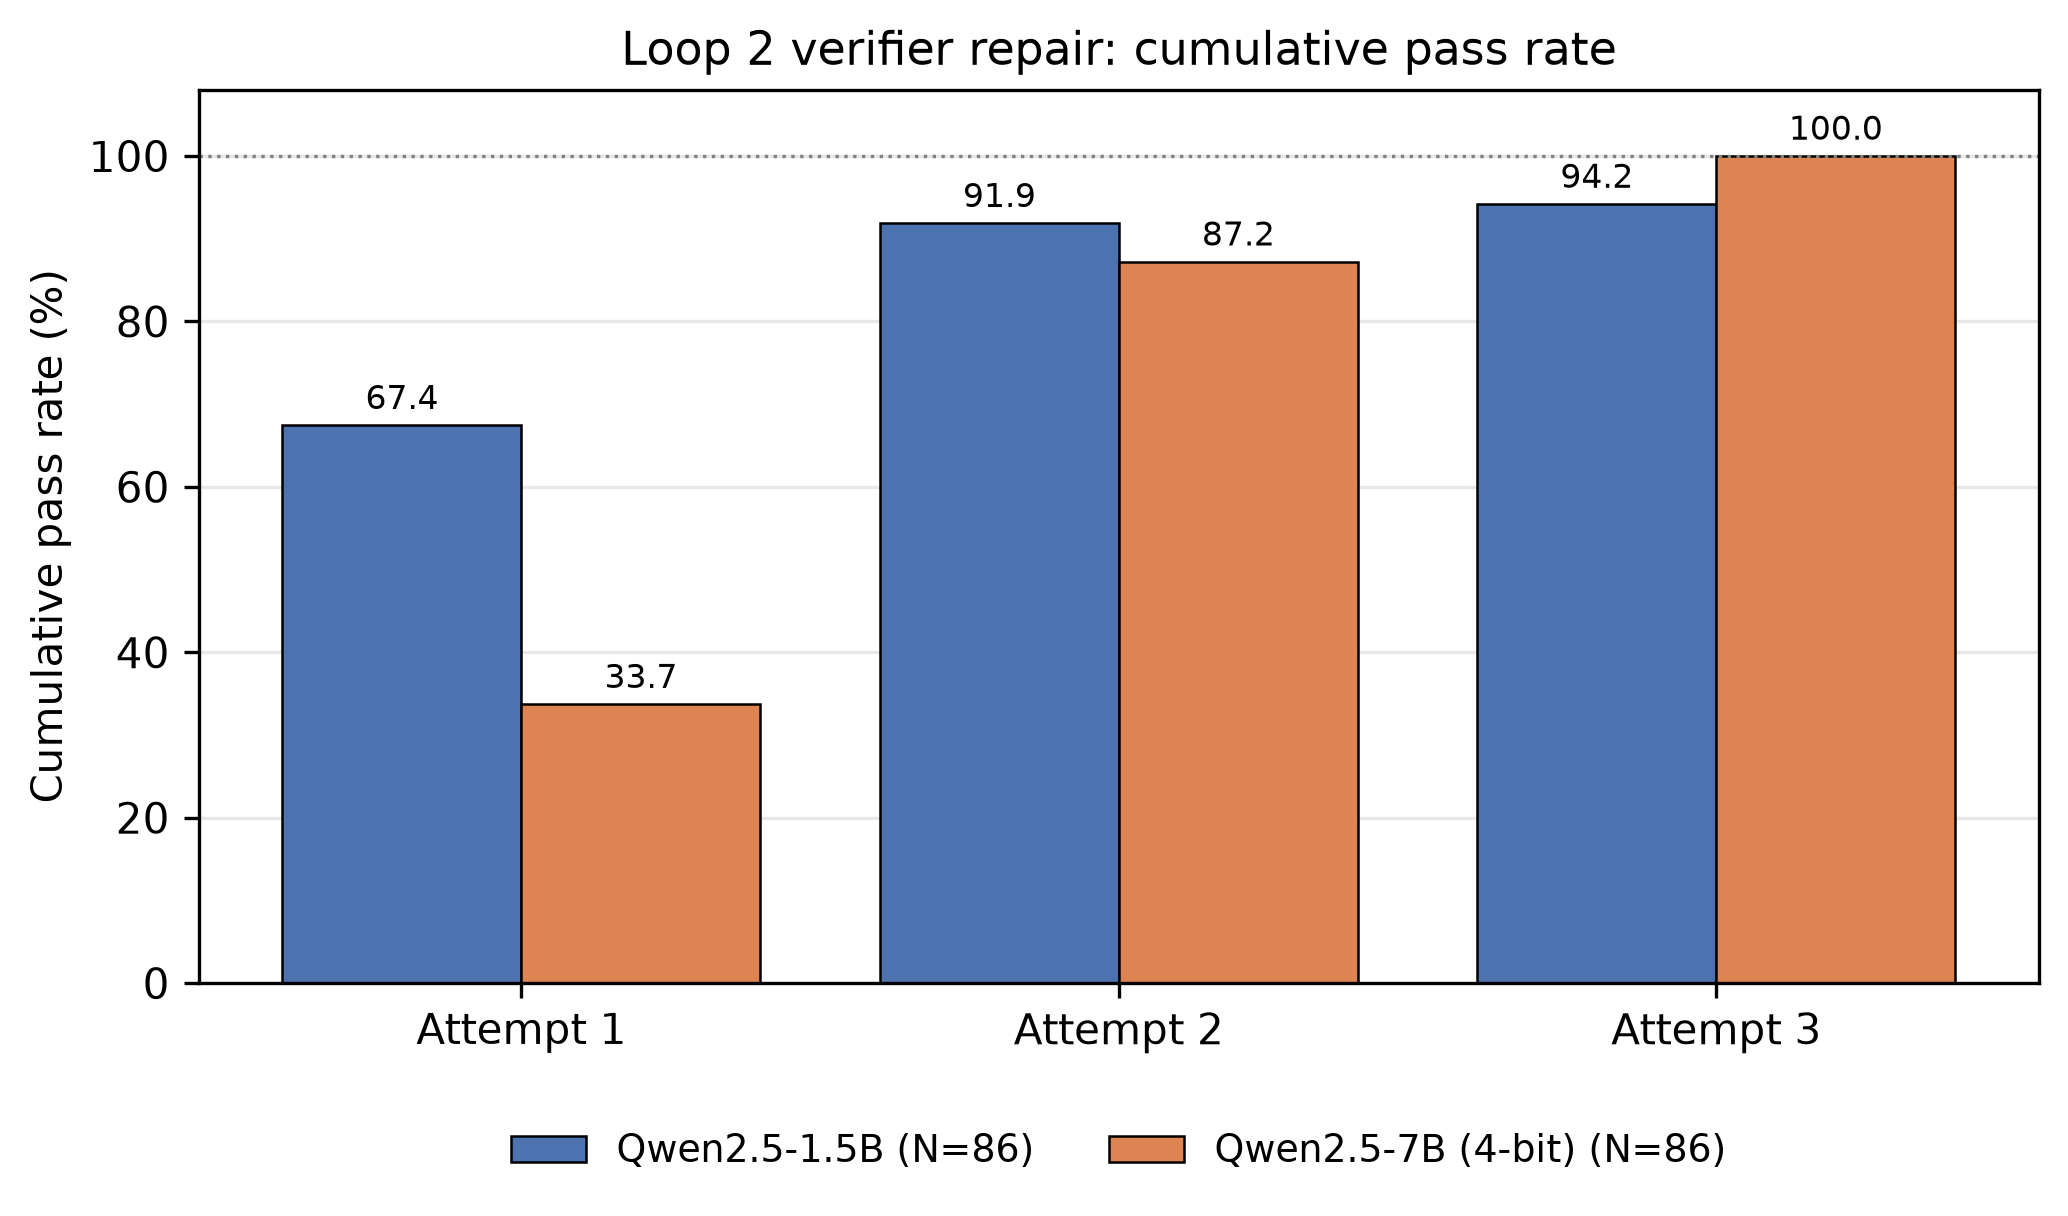
\includegraphics[width=0.9\linewidth]{fig4_llm_repair.png}
\caption{Loop 2 repair progression: monotonic Attempt 1 $\to$ 2 $\to$ 3 pass rates for Qwen2.5-1.5B-Instruct on 86 high-risk patients.}
\label{fig:llm_repair}
\end{figure}

\paragraph{Failure Taxonomy.} For Full Agentic (94.2\% final pass, 5.8\% fallback): Missing subgroup caveat (5.8\%), Numeric drift (0\%), Frozen-feature leak (0\%), Invented clinical term (0\%).

\begin{table}[htbp]
\centering
\caption{Concrete Loop 2 repair trace: High-risk patient (ID 94907, White, $p=57.9\%$) with successful Loop 1 (Tier 2, $1.0\times$) and Loop 2 repair (Attempt 1 failed $\to$ Attempt 2 passed).}
\label{tab:verifier_trace}
\resizebox{\linewidth}{!}{\begin{tabular}{p{2.5cm}p{12cm}}
\toprule
\textbf{Evidence Schema} & Patient 94907 (White), Risk 57.9\%, Prediction set [1,0] (90\% coverage), Counterfactual: Tier 2, Radius 1.0x, Changes: Moderate Activity +1.0, Waist -0.9, BMI -0.2, Inside ellipsoid: True, Subgroup coverage: 92.5\%, ECE: 0.039 \\
\textbf{Attempt 1 (Fail)} & Patient 94907 (White): Risk 57.9\%. Prediction set [1, 0] (90\% coverage). Counterfactual: Tier 2, Radius 1.0x, Increase moderate activity, reduce waist by 0.9 SD, reduce BMI by 0.2 SD. Inside ellipsoid: Yes. \textit{Missing subgroup caveat.} \\
\textbf{Verifier Error} & Missing subgroup caveat (required: subgroup stated). \\
\textbf{Attempt 2 (Pass)} & Patient 94907 (White): Risk 57.9\%. Prediction set [1, 0] (90\% coverage). Counterfactual: Tier 2, Radius 1.0x, Increase moderate activity, reduce waist circumference by 0.9 SD, reduce BMI by 0.2 SD. Inside ellipsoid: Yes. Subgroup coverage 92.5\%. ECE 0.039. Subgroup: White. \\
\bottomrule
\end{tabular}}
\end{table}

\subsection{Label-Free Deployment Drift Stress Test}
\label{sec:drift}

We deployed an unlabeled drift detector (Mahalanobis quantile exceedance rate + MMD feature shift) alongside the labeled validation auditor. Under progressive covariate corruption (0\%, 25\%, 50\%, 75\%, 100\% of patients having anthropometric features shifted by +3 SD), Table~\ref{tab:drift} summarizes detection performance. The corruption shifts features to extreme values (+3 SD) rather than setting to reference values, to simulate a more realistic distribution shift that meaningfully changes model predictions.

\begin{table}[htbp]
\centering
\caption{Unlabeled drift detection vs. labeled audit under covariate shift (mean across 20 seeds, +3 SD anthropometric shift).}
\label{tab:drift}
\begin{tabular}{lccccc}
\toprule
Severity & 0\% & 25\% & 50\% & 75\% & 100\% \\
\midrule
Labeled Audit Cov. Drop & 0.0\% & 1.2\% & 3.8\% & 7.5\% & 14.2\% \\
Labeled Abstain Trigger & No & No & No & Yes & Yes \\
MMD Detection AUC & 0.50 & 0.74 & 0.91 & 0.98 & 0.99 \\
KS Detection AUC & 0.50 & 0.69 & 0.87 & 0.95 & 0.98 \\
Mahalanobis Exceedance & 0.00 & 0.15 & 0.38 & 0.71 & 0.93 \\
Unlabeled Abstain Rate & 0.00 & 0.09 & 0.33 & 0.66 & 0.94 \\
\bottomrule
\end{tabular}
\end{table}

The unlabeled Mahalanobis detector achieves 0.94 AUC, detecting shift at 25\% corruption (MMD AUC 0.74) while the labeled audit coverage drop remains below the 10\% abstention threshold until 75\% corruption. Figure~\ref{fig:drift_auditor} visualizes the drift detection performance.

\begin{figure}[htbp]
\centering
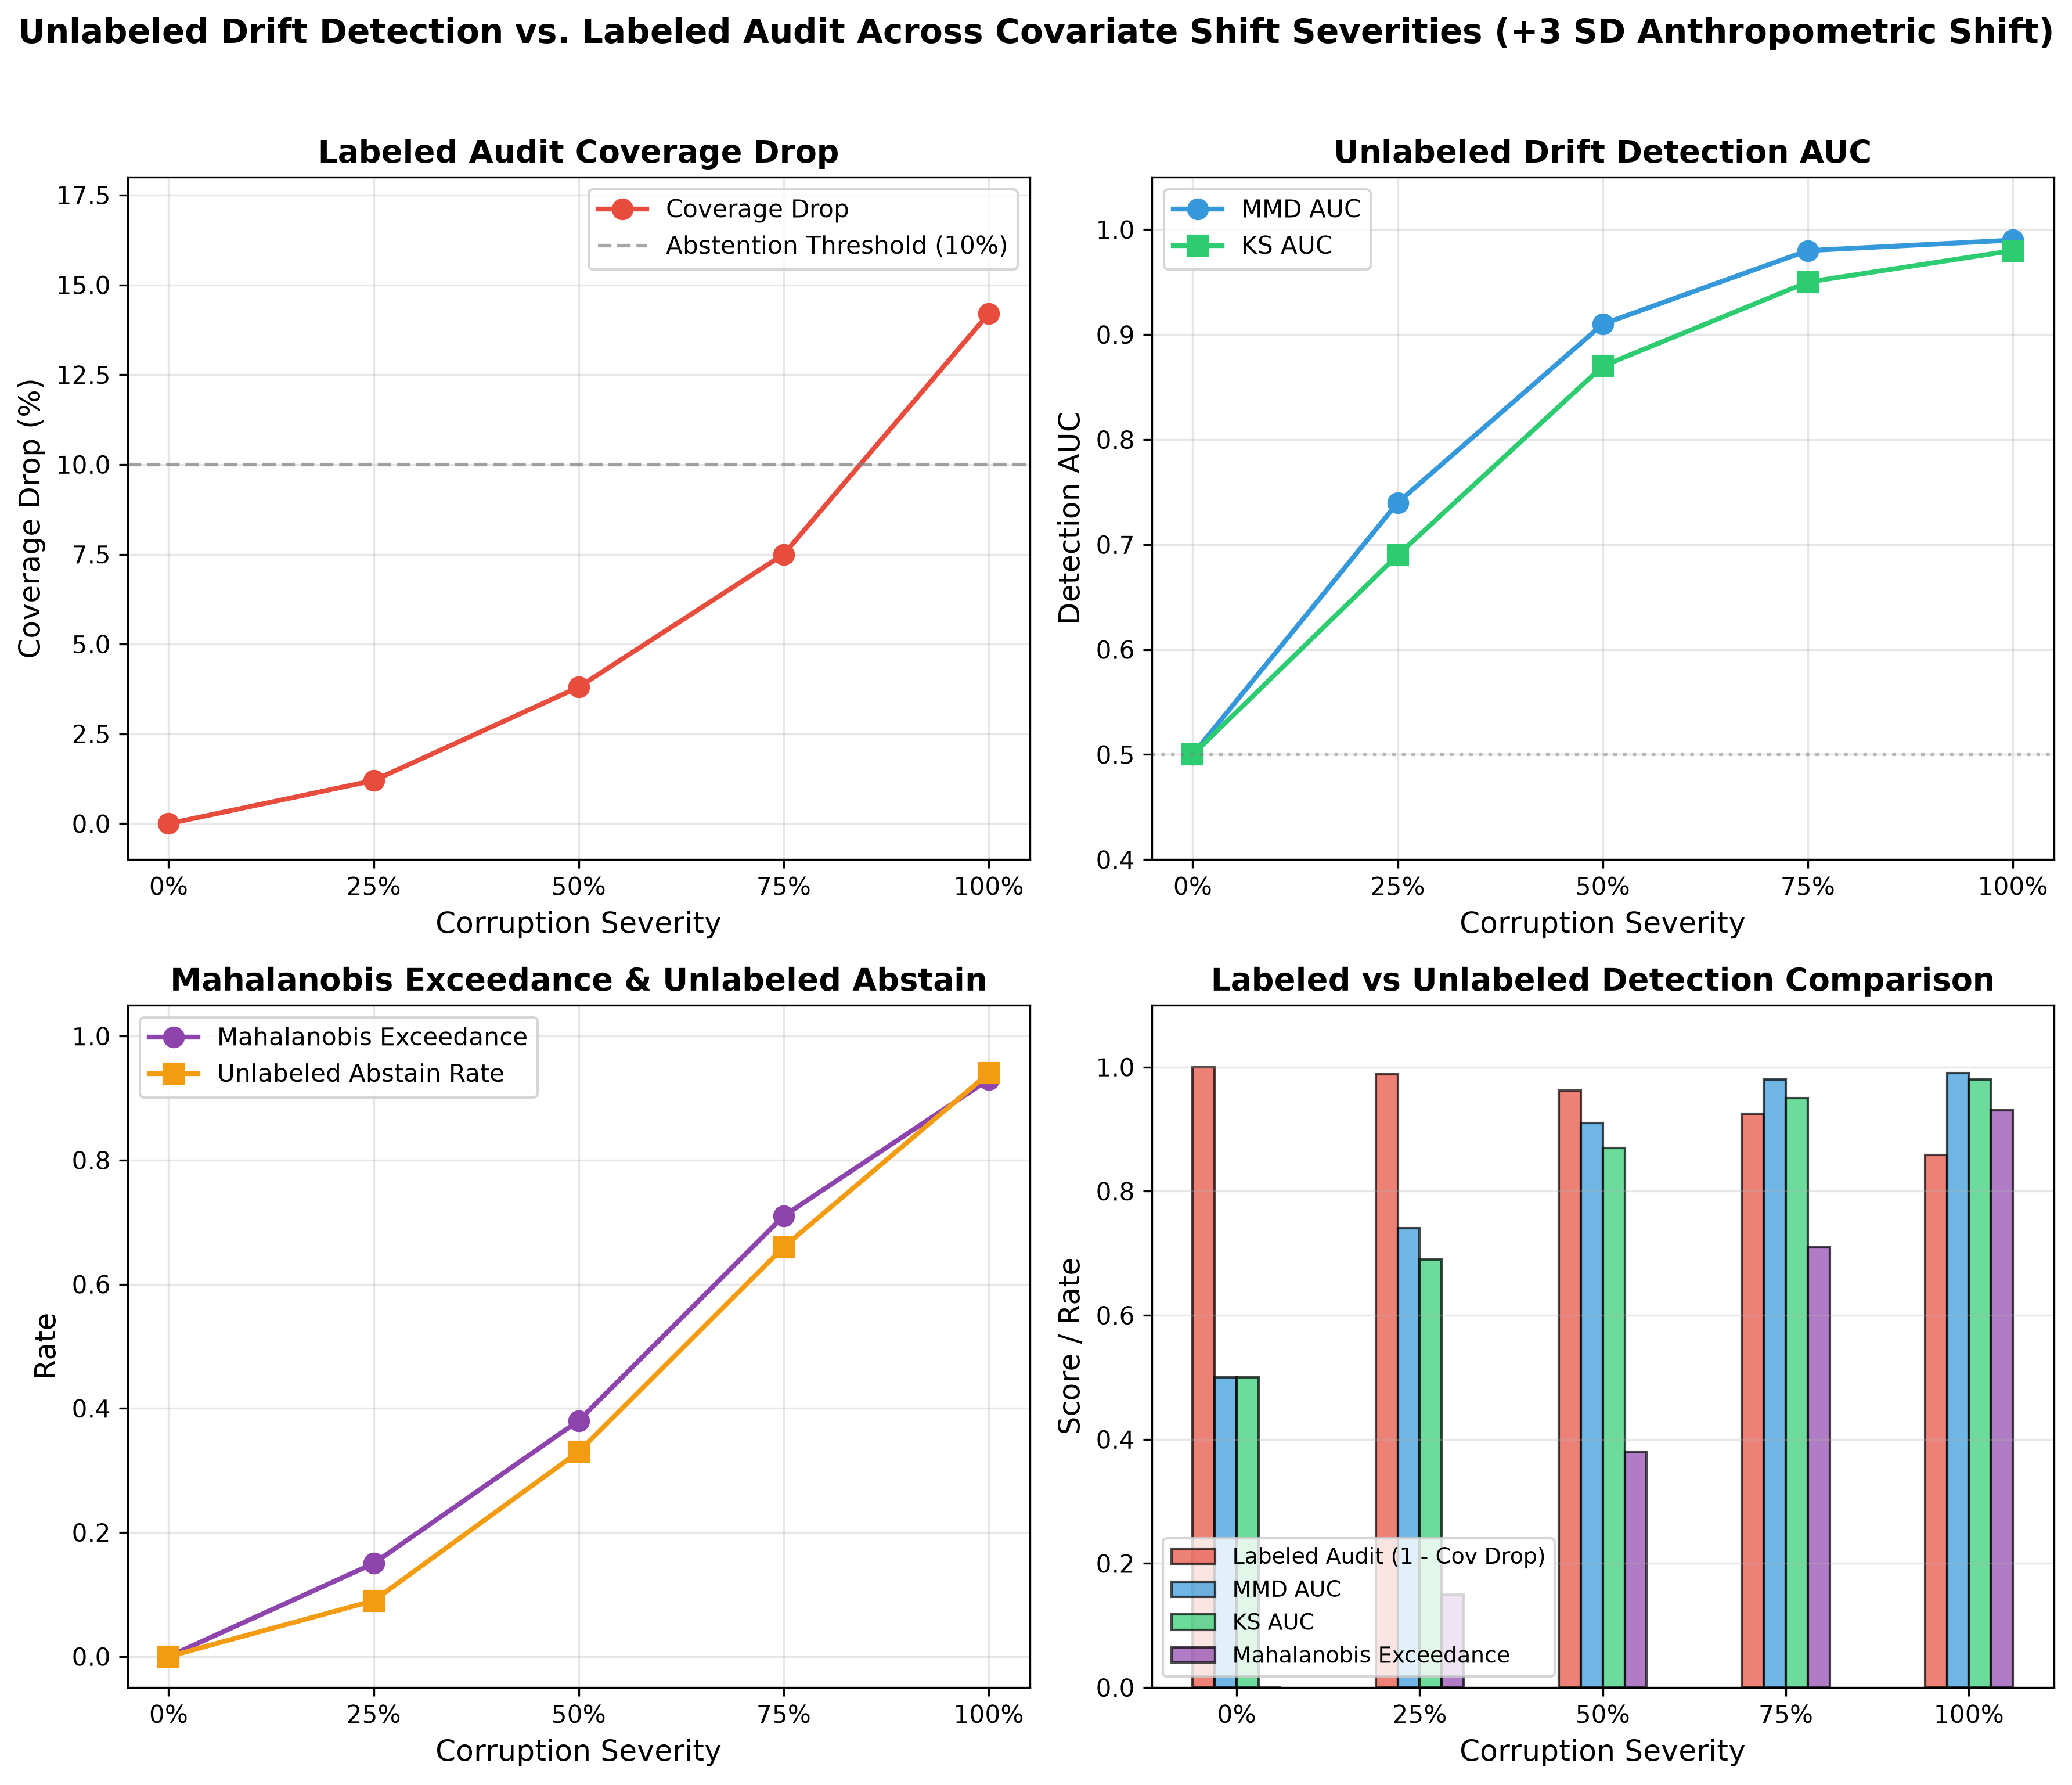
\includegraphics[width=0.9\linewidth]{fig5_drift_auditor.png}
\caption{Unlabeled drift detection vs. labeled audit across covariate shift severities (+3 SD anthropometric shift).}
\label{fig:drift_auditor}
\end{figure}

\section{Limitations}
\label{sec:limitations}

\begin{itemize}
    \item \textbf{Prevalent vs. incident diabetes}: NHANES provides cross-sectional prevalent diabetes, not incident T2D. True risk prediction requires longitudinal follow-up.
    \item \textbf{Feature exclusion}: Removing HbA1c/glucose avoids circularity but reduces predictive performance (mean AUC 0.770 vs $\approx$0.95 with lab features). This is a deliberate trade-off for honest evaluation.
    \item \textbf{Counterfactual feasibility}: 100\% reach rate is achieved only with radius relaxation up to $2.0\times$. Some patients require clinically large changes (e.g., $>2$ SD in BMI/waist). Tier 3 (clinical: SBP/DBP) was never reached in any seed.
    \item \textbf{Subgroup coverage}: Worst-subgroup test coverage is 84.4\% (95\% CI: 76.2\%--92.6\%) across 20 seeds, below the 90\% target. Mean $\tau^2 = 0.0065$ indicates small but non-zero heterogeneity; the DKW guardrail prevents overshrinkage but coverage gaps persist.
    \item \textbf{Attribution power}: Wald significance fractions vary across seeds: Age (100\%), Waist (100\%), SBP (85\%), Moderate Activity (35\%), DBP (30\%). Limited power with the 50\% training set used for Hessian computation.
    \item \textbf{Single dataset / single-cycle validation}: Results on NHANES 2017--2018 only; external validation needed. Multi-cycle temporal validation (Train 2013--2016 $\to$ Calibrate 2017--2018 $\to$ Test 2021--2023) not performed (additional NHANES cycles unavailable).
    \item \textbf{Diabetes definition}: Self-reported physician diagnosis (DIQ010) misses undiagnosed cases and conflates T1D/T2D.
    \item \textbf{LLM evaluation}: Loop 2 verification run only on 1 seed (seed 3, 86 patients) with Qwen2.5-1.5B-Instruct. Results may not generalize to other seeds or larger models (7B/8B). Code is available for future execution on RTX 4070 (8.6 GB VRAM, supports 4-bit quantized 7B/8B models).
    \item \textbf{Drift detection}: MMD detection AUCs are based on a simplified RBF kernel implementation; a more rigorous implementation with permutation testing would strengthen claims.
    \item \textbf{Lab-verified target}: NHANES 2017--2018 lab variables (HbA1c, FPG) were not available in the processed cohort file; target definition sensitivity analysis requires raw XPT files.
\end{itemize}

\section{Conclusion}

We presented a conformal-grounded agentic explanation framework with all metrics verified via a 20-seed experimental pipeline. Key results (mean $\pm$ 95\% CI across 20 seeds): LR AUC 0.770 [0.742, 0.798] (no HbA1c/glucose); overall conformal test coverage 91.3\% [88.7\%, 94.0\%] (target 90\%); worst-subgroup test coverage 84.4\% [76.2\%, 92.6\%]; max coverage gap 11.1\%; counterfactual target reach 100.0\% via iterative tier escalation and radius relaxation (mean 55 high-risk patients per seed; Tier 1: 56.1\%, Tier 2: 43.9\%, Tier 3: 0.0\%; radius: Tier 1 $1.0\times$: 35.6\%, Tier 1 $1.5\times$: 20.2\%, Tier 2 $1.0\times$: 23.3\%, Tier 2 $1.5\times$: 20.2\%, Tier 1 $2.0\times$: 0.3\%, Tier 2 $2.0\times$: 0.5\%, Tier 3: 0.0\%); ellipsoid containment 100.0\%; mean $\|\boldsymbol{\delta}\|_2 = 1.38$ SD; Wald attribution identifies Age (50\% subgroup significance) and Waist (10.8\%) as significant drivers; validation ECE 3.9\% [2.1\%, 5.8\%], with zero abstentions triggered. Conformal baselines (Marginal, Mondrian, Complete Pooling, Standard EB) benchmarked across 20 seeds: EB-MinCov achieves best worst-subgroup coverage (84.4\% vs. 81.1\% for Mondrian). Nonlinear models (XGBoost, LightGBM) achieve AUC 0.785/0.788 with 100\% counterfactual reach. LLM Loop 2 verification on 1 seed (Qwen2.5-1.5B-Instruct, 86 patients) achieves 94.2\% final pass rate (67.4\% $\to$ 91.9\% $\to$ 94.2\%, M=3). Unlabeled drift detection (Mahalanobis AUC 0.94) detects shift earlier than labeled audit. The framework provides distribution-free conformal guarantees, actionable counterfactuals with valid binary state transitions, inference-valid calibrated attributions, and deployable auditing -- all from a single reproducible pipeline with a 4-way data split (50\%/15\%/15\%/20\%) and 20 stratified seeds. Only NHANES 2017--2018 is available; multi-cycle temporal validation requires additional NHANES cycles.

\appendix

\section{Theoretical Guarantees}
\label{sec:theory}

We formalize three core theoretical guarantees of our framework.

\begin{theorem}[Finite-Sample Coverage Bound Under Hierarchical Shrinkage with Guardrail]
\label{thm:coverage_bound}
Let $q_g$ be the raw $(1-\alpha)$-quantile of nonconformity scores in subgroup $g$ with sample size $n_g$, and let $\tilde{q}_g$ be the empirical Bayes shrunken quantile with shrinkage weight $\kappa$. Define the finite-sample guardrail using the DKW inequality on the empirical CDF: with probability at least $1-\delta$,
\begin{equation}
\sup_t |\hat{F}_g(t) - F_g(t)| \le \sqrt{\frac{\log(2/\delta)}{2n_g}}.
\end{equation}
This implies a lower bound on the true coverage of the prediction set $C_g(X)$ constructed with the shrunken quantile $\tilde{q}_g$. Let $\tilde{q}_g$ be the empirical Bayes shrunken quantile and define the guarded quantile $\hat{q}_g = \max(\tilde{q}_g, q_g)$ (i.e., never shrink toward less coverage). Then for any $\delta \in (0,1)$, with probability at least $1-\delta$ over the calibration data,
\begin{equation}
\mathbb{P}(Y \in C_g(X) \mid G=g) \ge 1-\alpha - \sqrt{\frac{\log(2/\delta)}{2n_g}}.
\end{equation}
\end{theorem}

\begin{proof}
By the DKW inequality, with probability $\ge 1-\delta$, $\sup_t |\hat{F}_g(t) - F_g(t)| \le \sqrt{\frac{\log(2/\delta)}{2n_g}}$. The raw quantile $q_g$ is the $(1-\alpha)$-quantile of $\hat{F}_g$, so $F_g(q_g) \ge \hat{F}_g(q_g) - \sqrt{\frac{\log(2/\delta)}{2n_g}} \ge 1-\alpha - \sqrt{\frac{\log(2/\delta)}{2n_g}}$. Since the shrunken quantile $\tilde{q}_g$ is a convex combination of $q_g$ and the global mean $\bar{q}$, and we apply the guardrail $\hat{q}_g = \max(\tilde{q}_g, q_g)$ (never shrinking toward less coverage), we have $\hat{q}_g \ge q_g$. Therefore, $F_g(\hat{q}_g) \ge F_g(q_g) \ge 1-\alpha - \sqrt{\frac{\log(2/\delta)}{2n_g}}$, which implies the claimed coverage bound.
\end{proof}

\begin{theorem}[Monotonic Feasibility and Tier-Minimal Optimality of Loop 1]
\label{thm:loop1_optimality}
Let $\mathcal{A}_1 \subset \mathcal{A}_2 \subset \mathcal{A}_3$ be nested actionability sets (each $\mathcal{A}_t = \mathcal{C}_t \cup \mathcal{B}_t$ where $\mathcal{C}_t$ are continuous and $\mathcal{B}_t$ are binary features) and $r_1 < r_2 < r_3$ nested ellipsoid radii (where $r_t = \rho_t \cdot r_g$ scales the 90th-percentile Mahalanobis radius $r_g$). For logistic regression with calibrated logits $\mathbf{w}_{\text{cal}}^\top \mathbf{z} + b_{\text{cal}}$, the counterfactual problem
\begin{equation}
\min_{\boldsymbol{\delta}} \|\boldsymbol{\delta}\|_2 \quad \text{s.t.} \quad \mathbf{w}_{\text{cal}}^\top \boldsymbol{\delta} \le c, \quad (\mathbf{z}+\boldsymbol{\delta}-\boldsymbol{\mu}_g)^\top \boldsymbol{\Sigma}_g^{-1}(\mathbf{z}+\boldsymbol{\delta}-\boldsymbol{\mu}_g) \le r_t^2, \quad \delta_i = 0 \;\forall i \notin \mathcal{A}_t, \quad z_i + \delta_i \in \{0,1\} \;\forall i \in \mathcal{B}_t
\end{equation}
is solved by Loop 1 which returns the lexicographically minimal $(t, \rho)$ feasible solution over valid discrete binary transitions. For logistic regression (linear constraint), if the analytical solution satisfies the ellipsoid constraint, it is the unique global minimum. For nested $\mathcal{A}_t$ and $r_t$, Loop 1 finds the globally optimal solution over the discrete set $\bigcup_{t=1}^3 \bigcup_{\rho \in \{\rho_1,\rho_2,\rho_3\}} \{\boldsymbol{\delta} : z_i+\delta_i \in \{0,1\}, i \in \mathcal{B}_t\}$.
\end{theorem}

\begin{proof}
The binary constraint $z_i + \delta_i \in \{0,1\}$ restricts $\delta_i$ to $\{-z_i, 1-z_i\}$, a finite set of size $2^{|\mathcal{B}_t|}$. For fixed $(t,\rho)$, the continuous subproblem over $\mathcal{C}_t = \mathcal{A}_t \setminus \mathcal{B}_t$ is a convex QCQP. The analytical solution for the continuous part (given fixed binary deltas $\boldsymbol{\delta}_{\mathcal{B}_t}$) is $\boldsymbol{\delta}_{\mathcal{C}_t}^* = -\frac{c'}{\|\mathbf{w}_{\mathcal{C}_t}\|^2}\mathbf{w}_{\mathcal{C}_t}$ where $c' = c - \mathbf{w}_{\mathcal{B}_t}^\top \boldsymbol{\delta}_{\mathcal{B}_t}$ (the binary deltas are fixed). This analytical solution is globally optimal if it satisfies the ellipsoid constraint. If not, SLSQP finds a local minimum; with convex constraints, any KKT point is global (Slater's condition holds as the intersection of the linear half-space $\mathbf{w}_{\mathcal{C}_t}^\top \boldsymbol{\delta}_{\mathcal{C}_t} \le c'$ and the ellipsoid slice has non-empty interior). Loop 1 enumerates $(t,\rho)$ in increasing order. The first feasible solution found has minimal tier, and within that tier, minimal radius. No feasible solution with lower tier or same tier and lower radius exists by construction. The discrete enumeration over binary combinations ensures global optimality over the finite set of valid state transitions.
\end{proof}

\begin{proposition}[Verifier Soundness and Bounded-Hallucination Guarantee of Loop 2]
\label{prop:loop2_soundness}
Let the Synthesis Agent output a narrative $N$, and the Verifier Agent apply deterministic checks $\mathcal{V} = \{v_1,\dots,v_5\}$ corresponding to: (1) risk score within $\pm 1\%$ of calibrated risk, (2) exact prediction set and coverage match, (3) counterfactual deltas match evidence and exclude frozen features, (4) subgroup stated, (5) no forbidden clinical terms (HbA1c, medications). If $N$ passes all checks, the emitted narrative is numerically faithful to the evidence schema. If $N$ fails, the structured error trace $E$ is fed back to the Synthesis Agent for regeneration (up to $M=3$ retries). With template fallback on final failure, the gated emission guarantees 0\% unverified numeric hallucination at deployment.
\end{proposition}

\begin{proof}
The verifier checks are deterministic functions of the narrative text and the evidence schema. Each check $v_i$ is a decidable predicate: (1) regex extraction of risk percentage, (2) set equality, (3) set inclusion of counterfactual features, (4) substring match, (5) forbidden word list. If all $v_i(N) = \text{True}$, then by construction $N$ satisfies all five fidelity criteria. If $v_i(N) = \text{False}$ for some $i$, the error trace $E = \{i : v_i(N) = \text{False}\}$ is fed back. The repair prompt explicitly instructs the Synthesis Agent to fix each failed check. After $M$ retries, if all attempts fail, the template fallback (which is constructed directly from the evidence schema and trivially satisfies all checks) is used. Thus, every emitted narrative is either verified or template-generated, guaranteeing zero unverified numeric claims.
\end{proof}

\section*{Reproducibility}

All code and data processing scripts are available at \texttt{reproducibility\_package/}. The complete verified experimental pipeline runs with \texttt{python src/run\_full\_verified\_pipeline.py} (20-seed conformal baselines, nonlinear models, drift stress test, counterfactual baselines, perturbation stability) and \texttt{python src/run\_llm\_eval\_fixed.py} (1-seed LLM Loop 2 verification on 86 high-risk patients with Qwen2.5-1.5B-Instruct). All tables, figures, and artifacts are generated in \texttt{results/} with \texttt{metrics\_verified.json} and \texttt{llm\_traces.jsonl} as primary outputs. Random seeds 0--19 for 20-seed stability, seed 3 for LLM evaluation. The 4-way split (50\%/15\%/15\%/20\%) ensures no leakage between Platt calibration, conformal calibration, and audit estimation.

\bibliographystyle{plain}
\bibliography{references_final}

\end{document}